\documentclass{report}

\newcommand{\hlc}[2][yellow]{ {\sethlcolor{#1} \hl{#2}} }

\usepackage[T1]{fontenc}
\usepackage[utf8]{inputenc}
\usepackage{times}

\usepackage[font=small,labelfont=bf,tableposition=top]{caption}
\usepackage{graphicx}
\usepackage{natbib} 

\usepackage{amsmath}
\usepackage{amsfonts}
\usepackage{amssymb}
\usepackage{color, soul}
\usepackage{hyperref}
\usepackage{algorithmicx}
\usepackage{algpseudocode}
\usepackage{subfigure}
\usepackage{stmaryrd}

\renewcommand{\vec}[1]{\boldsymbol{{#1}}} 
\newcommand{\duesoon}[1]{{\sethlcolor{green}\hl{#1}}}
\usepackage{mathrsfs}


\newtheorem{theorem}{Theorem}
\newtheorem{acknowledgement}[theorem]{Acknowledgement}
\newtheorem{algorithm}[theorem]{Algorithm}
\newtheorem{axiom}[theorem]{Axiom}
\newtheorem{case}[theorem]{Case}
\newtheorem{claim}[theorem]{Claim}
\newtheorem{conclusion}[theorem]{Conclusion}
\newtheorem{condition}[theorem]{Condition}
\newtheorem{conjecture}[theorem]{Conjecture}
\newtheorem{corollary}[theorem]{Corollary}
\newtheorem{criterion}[theorem]{Criterion}
\newtheorem{definition}[theorem]{Definition}
\newtheorem{example}[theorem]{Example}
\newtheorem{exercise}[theorem]{Exercise}
\newtheorem{lemma}[theorem]{Lemma}
\newtheorem{notation}[theorem]{Notation}
\newtheorem{problem}[theorem]{Problem}
\newtheorem{proposition}[theorem]{Proposition}
\newtheorem{remark}[theorem]{Remark}
\newtheorem{solution}[theorem]{Solution}
\newtheorem{summary}[theorem]{Summary}
\newenvironment{proof}[1][Proof]{\textbf{#1.} }{\ \rule{0.5em}{0.5em}}

\newtheorem{guess}{Definition}
\newcommand{\comment}[1] {}
\newcommand{\Norder} {N}
\newcommand{\order}{\mathcal{O}}
\newcommand{\Npoints} {N_p}
\newcommand{\Nfaces} {N_{f}}
\newcommand{\Nelements} {N_e}

\newcommand{\eps}{\varepsilon}
\newcommand{\Dweak}{\wt{D}}
\newcommand{\diff}[2] {\frac{\partial #1}{\partial #2}}
\newcommand{\dxx}[2] {\frac{\partial^2 #1}{\partial {#2}^2}}
\newcommand{\difft}[2] {\frac{d #1}{d #2}}
\newcommand{\dxxt}[2] {\frac{d^2 #1}{d {#2}^2}}
\newcommand{\lagrange}[1] {\frac{d #1}{dt}}
\newcommand{\lebesgue}{\parallel I \parallel}
\newcommand{\polysp}{\mathcal{P}_N}
\newcommand{\laplacian}{\nabla^2}
\newcommand{\divergence}{\nabla \cdot}
\newcommand{\inte}{\int_{\mbox{\footnotesize ${\Omega_e}$}}}
\newcommand{\intb}{\int_{\mbox{\footnotesize ${\Gamma_e}$}}}
\newcommand{\intce}{\int_{\mbox{\footnotesize ${\widehat{\Omega}_e}$}}}
\newcommand{\intcb}{\int_{\mbox{\footnotesize ${\widehat{\Gamma}_e}$}}}
\newcommand{\intg}{\int_{\mbox{\footnotesize ${\Omega}$}}}
\newcommand{\intgb}{\int_{\mbox{\footnotesize ${\Gamma}$}}}
\newcommand{\intv}{\int_{\mbox{\footnotesize ${\sigma}$}}}
\newcommand{\sumv}{\sum_{K=1}^{N_{\mathrm{lev}}}}
\newcommand{\sumk}{\sum_{L=1}^{K}}
\newcommand{\sumN}{\sum_{i=1}^{N+1}}
\newcommand{\half}{\frac{1}{2}}
\newcommand{\inti}{\int_{\mbox{\footnotesize\sf I}}}
\newcommand{\intbd}{\oint_{\mbox{\footnotesize ${\delta}$\sf D}}}
\newcommand{\intbi}{\oint_{\mbox{\footnotesize ${\delta}$\sf I}}}
\newcommand{\ldnorm}[1]{\left\| #1 \right\|_{\mbox{\footnotesize \sf D}} }
\newcommand{\lonorm}[1]{\left\| #1 \right\|_{\Omega}}
\newcommand{\spc}[1]{\mbox{\sf #1}}
\newcommand{\ope}[1]{{\cal #1}}
\newcommand{\mt}[1]{{\rm #1}}
\newcommand{\dis}{\displaystyle}
\newcommand{\ve}{\varepsilon}
\newcommand{\ov}{\overline}
\newcommand{\wt}{\widetilde}
\newcommand{\wh}{\widehat}
\newcommand{\Dhat}{\widehat{D}}
\newcommand{\be}{\begin{equation}}
\newcommand{\ee}{\end{equation}}
\newcommand{\bea}{\begin{eqnarray*}}
\newcommand{\eea}{\end{eqnarray*}}
\newcommand{\Jace}{J^{(e)}}
\newcommand{\Jacl}{J^{(l)}}
\def\bepsilon{\mbox{\boldmath $\epsilon $}}
\def\bpsi{\mbox{\boldmath $\psi $}}
\def\bphi{\mbox{\boldmath $\phi $}}
\def\bmu{\mbox{\boldmath $\mu $}}
\def\Et{ \tilde{E} }
\def\Ht{ \tilde{H} }
\def\sdot{ \dot{\sigma} }

\newcommand{\fstar}{f^{(*)}}

\DeclareMathOperator{\Span}{span}
\DeclareMathOperator{\Dim}{dim}

\newcommand{\polyquad}{\mathcal{Q}_{N}}
\newcommand{\polyP}{\mathcal{P}_{N}}
\newcommand{\polyPnpm}{\mathcal{P}_{(N+M)}}
\newcommand{\polyPd}{\mathcal{P}_{d}}
\newcommand{\polyPnm}{\mathcal{P}_{N,M}}
\newcommand{\polyPn}{\mathcal{P}_{N,0}}
\newcommand{\transpose}{^{\mathcal{T}}}

\newcommand{\vecQ}{\vec{Q}}
\newcommand{\vecQe}{\vec{Q}^{(e)}}
\newcommand{\vecFe}{\vec{\mathcal{F}}^{(e)}}
\newcommand{\statevec}{\vec{Y}}
\newcommand{\statevecN}{\vec{Y}_N^{(e)}}
\newcommand{\statestage}{\vec{\mathcal{Y}}}
\newcommand{\Ftensor}{\vec{F}(\qvector)}
\newcommand{\FtensorN}{\vec{F}\left( \qvectorN \right)}
\newcommand{\FtensorStar}{\vec{F}\left( \qvector_N^{(e,k)} \right)}
\newcommand{\Svector}{S(\qvector)}
\newcommand{\SvectorN}{S \left( \qvectorN \right)}
\newcommand{\qref}{\vec{q}_0}
\newcommand{\qvectorb}{\vec{q}_b}
\newcommand{\qtt}{\vec{q}_{tt}}
\newcommand{\qhat}{\widehat{\vec{q}}}
\newcommand{\qhatb}{\widehat{\vec{q}}_b}
\newcommand{\qelem}{q^{(e)}}
\newcommand{\rhoref}{\rho_0}
\newcommand{\piref}{\pi_0}
\newcommand{\Thetaref}{\Theta_0}
\newcommand{\Gref}{G_0}
\newcommand{\Tref}{T_0}
\newcommand{\thetaref}{\theta_0}
\newcommand{\Pref}{{P}_0}
\newcommand{\Eref}{{E}_0}
\newcommand{\Href}{{h}_0}
\newcommand{\rhohat}{\widehat{\rho}}
\newcommand{\pihat}{\widehat{\pi}}
\newcommand{\Phat}{\widehat{P}}
\newcommand{\uvechat}{\widehat{{\mbox{\boldmath$u$\unboldmath}}}}
\newcommand{\uhathat}{\widehat{\widehat{{\mbox{\boldmath$u$\unboldmath}}}}}
\newcommand{\Uhat}{\widehat{{\mbox{\boldmath$U$\unboldmath}}}}
\newcommand{\Uhathat}{\widehat{\widehat{{\mbox{\boldmath$U$\unboldmath}}}}}
\newcommand{\thetahat}{\widehat{\theta}}
\newcommand{\Thetahat}{\widehat{\Theta}}
\newcommand{\Ehat}{\widehat{E}}
\newcommand{\uhat}{\widehat{u}}
\newcommand{\vhat}{\widehat{v}}
\newcommand{\what}{\widehat{w}}
\newcommand{\pitt}{\pi_{tt}}
\newcommand{\rhott}{\rho_{tt}}
\newcommand{\Ett}{E_{tt}}
\newcommand{\Utt}{\vec{U}_{tt}}
\newcommand{\uvectt}{\vec{u}_{tt}}
\newcommand{\utt}{u_{tt}}
\newcommand{\vtt}{v_{tt}}
\newcommand{\wtt}{w_{tt}}
\newcommand{\Ptt}{P_{tt}}
\newcommand{\vecPtt}{\vec{P}_{tt}}
\newcommand{\Thetatt}{\Theta_{tt}}
\newcommand{\thetatt}{\theta_{tt}}
%Projector Matrices
\newcommand{\projmatrix}{\vec{\mathcal{P}}}
\newcommand{\qmatrix}{\vec{\mathcal{Q}}}
\newcommand{\pcmatrix}{\vec{\mathcal{P}}_C}
\newcommand{\Cmatrix}{\left(\vec{\mathcal{C}}^{(e,f)}\right)\transpose}
\newcommand{\Dmatrix}{\vec{D}^{(e)}}
\newcommand{\Dwmatrix}{\wt{\vec{D}}^{(e)}}
\newcommand{\Mmatrix}{M^{(e)}}
\newcommand{\Fmatrix}{\vec{F}^{(e,l)}}
\newcommand{\Gmatrix}{\mathcal{G}}
\newcommand{\Umatrix}{\mathcal{U}^{(e,f)}}
\newcommand{\amatrix}{\vec{\mathcal{A}}}
\newcommand{\rmatrix}{\vec{\mathcal{R}}}
%Vectors
\newcommand{\nvector}{\wh{\vec{n}}_{\Gamma}}
\newcommand{\nhat}{\wh{\vec{n}}}
\newcommand{\ivector}{\wh{\vec{i}}}
\newcommand{\jvector}{\wh{\vec{j}}}
\newcommand{\kvector}{\wh{\vec{k}}}
\newcommand{\rvector}{\wh{\vec{r}}}
\newcommand{\svector}{\wh{\vec{s}}}
\newcommand{\tvector}{\wh{\vec{t}}}
\newcommand{\vvector}{\wh{\vec{v}}}
\newcommand{\Qvector}{\vec{Q}}
%Vectors
\newcommand{\ur}{{u}^{(r)}}
\newcommand{\us}{{u}^{(s)}}
\newcommand{\ut}{{u}^{(t)}}
\newcommand{\urtt}{{u}_{tt}^{(r)}}
\newcommand{\ustt}{{u}_{tt}^{(s)}}
\newcommand{\uttt}{{u}_{tt}^{(t)}}
\newcommand{\urhat}{\widehat{u}^{(r)}}
\newcommand{\ushat}{\widehat{u}^{(s)}}
\newcommand{\uthat}{\widehat{u}^{(t)}}
%Other Operators
\newcommand{\grad}{\vec{\nabla}}
\newcommand{\Grad}{\vec{\nabla}}
\newcommand{\Dskew}{\mathcal{D}}

\def\bepsilon{\mbox{\boldmath $\epsilon $}}
\def\bpsi{\mbox{\boldmath $\psi $}}
\def\bphi{\mbox{\boldmath $\phi $}}
\def\bmu{\mbox{\boldmath $\mu $}}
\def\Et{ \tilde{E} }
\def\Ht{ \tilde{H} }
\def\sdot{ \dot{\sigma} }
%\renewcommand{\thetable}{\Roman{table}}
%\renewcommand{\thefigure}{\arabic{figure}}

%\DeclareMathOperator{\Span}{span}
%\DeclareMathOperator{\Dim}{dim}

%Editing Commands
\newcommand{\here}{ \textcolor{red}{YOU ARE HERE}}

%Time-Integration
\newcommand{\dt}{{\Delta t}}
\newcommand\ST{\rule[-0.75em]{0pt}{2em}}
\newcommand{\Sfunction}{\mathcal{S}}
\newcommand{\Lfunction}{\mathcal{L}}
\newcommand{\Nfunction}{\mathcal{N}}

%DG Operators
\newcommand{\average}[1]{ \left\{ #1 \right\} }
\newcommand{\jump}[1]{ \llbracket #1 \rrbracket }

%HDG Matrices
\newcommand{\CCmatrix}{\mathcal{C}^{(e,k)}}
\newcommand{\Jmatrix}{\mathcal{J}^{(e,k)}}
\newcommand{\DDmatrix}{\wt{D}^{(e)}}
\newcommand{\SSvector}{\mathcal{S}(q)}
\newcommand{\cghdg}{cg\underline{\hspace{0.15cm}}to\underline{\hspace{0.15cm}}hdg}
%\newcommand{\ul}{\underline{\hspace{0.15cm}}}
\newcommand{\RRmatrix}{\mathcal{R}}

%Clima specific variables
\newcommand{\etotal}{e^{\mathrm{tot}}}
\newcommand{\Etotal}{E^{\mathrm{tot}}}
\newcommand{\Fvector}{\vec{\mathcal{F}}}
\newcommand{\Pvector}{\vec{\mathcal{P}}}
\newcommand{\Fadv}{\vec{\mathcal{F}}^{\mathrm{adv}}}
\newcommand{\Fndf}{\vec{\mathcal{F}}^{\mathrm{ndf}}}
\newcommand{\Fdiff}{\vec{\mathcal{F}}^{\mathrm{diff}}}
\newcommand{\Tvector}{\vec{\mathcal{T}}}
\newcommand{\Source}{\vec{\mathcal{S}}}

\newcommand{\fxg}[1]{\textcolor{cyan}{FXG: #1}}


\usepackage[inline]{enumitem}


\title{Numerics of CLIMA Models} 
\author{}

\begin{document}

\maketitle
\tableofcontents

\hl{[simon]:  can we add a table of terms, and their corresponding symbols and function names in the code?}

\chapter{Space Discretization}

%\hl{2019/09/19: I (Jeremy) am working on rewriting this. Still have some things to add, so it should be seen as a work in progress\dots}

\section{Problem Formulation}

To describe the methods used to solve the governing equations numerically, we write the equations in the compact, $d$-dimensional balance law form 
\begin{equation}\label{e:eom_compact}
\diff{\vec{Y}}{t}  =  - \nabla \cdot \Fvector + \vec{\mathcal{S}}(\vec{Y}, \vec{x}, t),
\end{equation}
where $\vec{Y}$ is the \emph{state} vector, $\partial\vec{Y}/\partial t$ is the \emph{tendency} of the state vector, $\Fvector$ is the \emph{flux} vector, $\vec{\mathcal{S}}(\vec{Y})$ are \emph{sources}, and $\vec{x}$ and $t$ are the space and time coordinates. The flux vector is further subdivided into non-diffusive fluxes and diffusive fluxes (which depend on gradients of state variables),
\begin{equation}
    \Fvector = \Fnondiff\left(\vec{Y}, \vec{x}, t\right) + \Fdiff\left(\vec{Y}, \vec{\Sigma}, \vec{x}, t\right).
\end{equation}
Here, 
\begin{equation}
    \vec{\Sigma} = \diffusive(\vec{Y}, \nabla \gradvariables(\vec{Y}, \vec{x}, t), t)
\end{equation}
is an auxiliary variable that has been introduced to account for terms that depend on the gradient of the state vector $\vec{Y}$ (i.e., it is the auxiliary variable that represents the derivative of a quantity in the LDG formulation). The function $\gradvariables$ transforms the state prior to the variables to have the gradient taken, and the function $\diffusive$ is used to transform to the auxiliary variables. In principle $\diffusive$ could be applied in $\Fdiff$, but this formulation allows the most flexibility in terms of enforcing continuity of the solution, namely $\vec{\Sigma}$ should be the quantity that continuity is enforced on.

For the spatial discretization, we use variants of the discontinuous Galerkin (DG) method with tensor-product bases (see, e.g., \citealt{giraldo:2008a,abdi:2016}). We use hexahedral (cube) elements in three dimensions.  The nodal tensor-product DG methods are extremely accurate and efficient.  For example, using a basis comprised of $N$-th degree Lagrange polynomials results in approximately an accuracy of $\order(\Delta x^{N+1})$. Furthermore, using inexact integration results in a per-element complexity of $\order(N^{d+1})$ for constructing derivatives, where $d$ denotes the dimension of the space. For both the global and LES models, we use fully three-dimensional DG methods.

The domain is assumed to be embedded in a Cartesian coordinate system, which the coordinate vector has components $\vec{x} = (x_{1}, x_{2}, x_{3})$. Each discretization element has its own reference coordinate system, defined so that the element is a square (in 2D) or cube (in 3D). A point in the reference element is denoted as $\vec{\xi}$ with components $(\xi_{1}, \xi_{2}, \xi_{3})$.  It is important to note that $x_{3} \ne z$ if $z$ is taken to be height (the direction opposite to the gravitational acceleration).

% [No need for specific code references here, which may change.] Currently, in the CLIMA source\footnote{see
% \texttt{src/DGmethods/balanacelaw.jl} at
% \url{https://github.com/climate-machine/CLIMA/blob/master/src/DGmethods/balancelaw.jl}}
% the above functions are defined as
% \begin{table}[h]
%   \centering
%   \begin{tabular}{ll}
%     $\Fnondiff$       & \texttt{flux\_nondiffusive!}\\
%     $\Fdiff$          & \texttt{flux\_diffusive!}\\
%     $\gradvariables$  & \texttt{gradvariables!!}\\
%     $\diffusive$      & \texttt{diffusive!}\\
%     $\Source$         & \texttt{source!}\\
%   \end{tabular}
% \end{table}

\section{Finite Element Mesh}
In finite element methods, the domain is decomposed into a set of elements and
the solution is approximated in each element using a finite dimensional function
space. The solution approximation is constructed by requiring that the residual
is orthogonal (in some inner product) to the space of functions. In the
discontinuous Galerkin method, the choice of numerical method for CLIMA,
the space of functions is discontinuous across element boundaries as continuity
of the solution and boundary conditions are enforced weakly through the use of
numerical fluxes (similar to finite volume methods).

As is often done in finite elements, elements are mapped to a reference domain.
In the reference domain the elements have the domain ${[-1, 1]}^d$ where $d$ is
the dimensionality of the problem; thus in 2-D the reference element is a square
and in 3-D a cube. There is then a diffeomorphic mapping between each element in
the physical space and the reference space. Thus, for a single element $e$ the
mapping is of the form $\vec{x}^{(e)}(\vec{\xi})$ and its inverse is
$\vec{\xi}^{(e)}(\vec{x})$; note that each element will have a different mapping
function. These mapping must be accounted for when discretizing the equations
through the use of metric terms.

\section{Basis Functions}
On the reference element, the space of functions used is tensor-product
polynomials of degree $N$; the space of tensor-product polynomials of degree $N$
is denoted as $\mathbb{Q}^{N}(\hat{e})$ where $\hat{e} = {[-1, 1]}^d$ is the
reference element. In 3-D the solution inside the element is taken to be
\begin{align}
  \vec{Y}^{(e)}(\vec{\xi}, t) = \sum_{(i,j,k) = (0,0,0)}^{(N,N,N)}
  l_{i}(\xi_{1}) l_{j}(\xi_{2}) l_{k}(\xi_{3})
  \vec{Y}_{ijk}^{(e)}(t),
\end{align}
Here $l_{i}(\vec{x})$ are 1-D Lagrange polynomials associated with a set of
abscissae ${\{\hat{\xi}_{k}\}}_{k=0}^{N}$ (which should not be confused with
$\xi_{k}$ which is a component of $\vec{\xi}$). In terms of the physical
coordinate $\vec{x}$ the solution inside the element is then
\begin{align}
  \vec{Y}^{(e)}(\vec{\xi}^{(e)}(\vec{x}), t) = \sum_{(i,j,k) = (0,0,0)}^{(N,N,N)}
  l_{i}(\xi_{1}^{(e)}(\vec{x})) l_{j}(\xi_{2}^{(e)}(\vec{x}))
  l_{k}(\xi_{3}^{(e)}(\vec{x}))
  \vec{Y}_{ijk}^{(e)}(t).
\end{align}
Note that depending on the mapping $\vec{\xi}^{(e)}(\vec{x})$ the solution need
not be tensor product polynomial in the physical space.

\section{DG Formulation}
The discontinuous Galerkin scheme used in CLIMA is: for element $e$ find a
function $\vec{Y}^{(e)} \in \mathbb{Q}^{N}(\hat{e})$
and $\vec{\Sigma}^{(e)} \in \mathbb{Q}^{N}(\hat{e})$
such that
\begin{align}
  &\int_{e}
  \left(
  \vec{\Psi}^T \diff{\vec{Y}}{t}
  + \frac{1}{2}
  \left(
  \vec{\Psi}^{T} \nabla \cdot \Fnondiff
  -
  \nabla\vec{\Psi} \cdot
  \Fnondiff
  \right)
  -
  \nabla\vec{\Psi} \cdot
  \Fdiff
  \right)
  \label{eq:dg_formulation/governing_equations} \\\notag
  &\quad\quad\quad =
  \int_{e} \vec{\Psi}^T \Source
  -
  \int_{\partial e}
  \vec{\Psi}^{T}
  {\left(\nhat^{-} \cdot \Fdiff\right)}^{*}
  \\\notag
  &\quad\quad\quad\phantom{=}-
  \int_{\partial e}
  \vec{\Psi}^{T} \left(
  {\left(\nhat^{-} \cdot \Fnondiff\right)}^{*}
  - \frac{1}{2} \nhat^{-} \cdot {\left(\Fnondiff\right)}^{-}
  \right)
  ,\\
  &\int_{e}
  \left(
  \vec{\Phi}^T \vec{\Sigma}
  -
  \vec{\Phi}^T \diffusive(\vec{Y}, \nabla \gradvariables, t)
  \right)
  =
  \int_{\partial e} \vec{\Phi}^{T} \left(
  \diffusive^{*} - \diffusive\left(\vec{Y}^{-},
  \nhat^{-}\gradvariables^{-}, t\right)
  \right),
  \label{eq:dg_formulation/auxiliary_equations}
\end{align}
\hl{[simon]: is there a reason we write $\nhat^{-}$ instead of just $\vec{n}$? It would make it slightly cleaner.}\\
\hl{[jeremy]: main reason I did this is to make it clear that the normal is not with respect to the face, but the element. Some folks use a unique face normal for each face, whereas we define the normal with respect to the element on the minus side. I've seen it both ways in the literature.}
\fxg{We could use $\nhat$ with a statement that it is the normal on the interior side and use other notation when not the case.  It does break the symmetry a bit when we have both plus and minus sides in an equation. We can do away with the plus side normals entirely then. I'm OK either way. If we agree to remove plus and minuses from the normals, I can clean this up to reflect this change.} 

for all $\vec{\Psi} \in \mathbb{Q}^{N}(\hat{e})$ and $\vec{\Phi} \in
\mathbb{Q}^{N}(\hat{e})$.  Looking at these equations, it can be seen that we treat Eq.\ \eqref{eq:dg_formulation/governing_equations} in weak form\footnote{The \emph{weak} form means that we use integration by parts to move the gradient from the flux function to the basis function as shown in the volume integral ($e$) of Eq.\ \eqref{eq:dg_formulation/governing_equations}.} and Eq.\ \eqref{eq:dg_formulation/auxiliary_equations} in strong form \footnote{The \emph{strong} form means that we use a second integration by parts to move the gradient back to the flux function, which results in the extra term in the surface integral ($\partial e$) of Eq.\ \eqref{eq:dg_formulation/auxiliary_equations}.}. Here it is understood that $\Fnondiff =
\Fnondiff(\vec{Y}, t)$, $\Fdiff = \Fdiff(\vec{Y}, \vec{\Sigma}, t)$, and
$\gradvariables = \gradvariables(\vec{Y}, t)$. In the surface integrals, for any quantity $q$, the
terms $q^-$ are evaluated inside the element $e$, $q^+$ on the face neighbor, and $q^*$ are the numerical fluxes which enforce continuity of the solution
across element faces and are used to enforce boundary conditions. At
interior element faces the numerical flux functions have the following
dependencies:
\begin{align}
  {\left(\nhat^{-} \cdot \Fnondiff\right)}^{*}
  &=
  {\left(\nhat^{-} \cdot \Fnondiff\right)}^{*}
  \left(
  \vec{Y}^{-}, \vec{Y}^{+}, \nhat^{-}, t
  \right),\\
  %
  {\left(\nhat^{-} \cdot \Fdiff\right)}^{*}
  &=
  {\left(\nhat^{-} \cdot \Fdiff\right)}^{*}
  \left(
  \vec{Y}^{-}, \vec{Y}^{+}, \vec{\Sigma}^{-}, \vec{\Sigma}^{+}, \nhat^{-}, t
  \right),\\
  %
  \diffusive^{*} &=
  \diffusive^{*}\left(
  \vec{Y}^{-}, \vec{Y}^{+}, \nhat^{-}, t
  \right).
\end{align}


\begin{table}[htbp]
  \centering
  \begin{tabular}{cl}
    ${\left(\nhat^{-} \cdot \Fnondiff\right)}^{*}$ & \texttt{numerical\_flux\_nondiffusive!}\\
    ${\left(\nhat^{-} \cdot \Fdiff\right)}^{*}$    & \texttt{numerical\_flux\_diffusive!}\\
    $\diffusive^{*}$                               & \texttt{numerical\_flux\_gradient!}\\
  \end{tabular}
\end{table}

\section{Numerical Flux}
A variety of choices can be made for the numerical flux functions, and here we
outline the choices made by \citet{bassi:1997nse} which we follow in CLIMA.

The numerical flux for the non-diffusive flux\footnote{In \citet[Eq.
(10)]{bassi:1997nse} this is the function $\vec{h_{e}}$.} is set using the
Rusanov (or Local Lax-Friedrichs) flux:
\begin{equation}
  \left( \nhat^{-} \cdot \Fnondiff\right)^{*} =
  \frac{\nhat^{-}}{2} \cdot 
  \left[ \left(\Fnondiff\right) ^{+} +
  \left(\Fnondiff\right)^{-}
  -
  \lambda \nhat^{-} \left( \vec{Y}^{+} - \vec{Y}^{-} \right) 
  \right],
  \label{eq:nondiff_flux}
\end{equation}
\comment{
\begin{align}
  {\left(
  \nhat^{-} \cdot \Fnondiff\right)}^{*} =
  \frac{\nhat^{-}}{2} \cdot 
  \left[
  {\left(\Fnondiff\right)}^{+} +
  {\left(\Fnondiff\right)}^{-}
  -
  \lambda \nhat^{-} \left( \vec{Y}^{+} - \vec{Y}^{-} \right) 
  \right],
  \label{eq:nondiff_flux}
\end{align}
}
where $\lambda = \lambda(\vec{Y}^{-}, \vec{Y}^{+})$ is an estimate of the
maximum wavespeed, i.e., the maximum eigenvalue of the Jacobian of the flux
function $\Fnondiff$. 
%Here the subscript $+$ denotes the value on the face of the opposing element. 
As noted in \citet{bassi:1997nse} other choices of the
non-diffusive numerical flux are possible such as Roe, Engquist-Osher, HLLE
(Harten, Lax, Van Leer, Einfeldt), and exact Godunov.

The numerical flux for the diffusive flux\footnote{In \citet[Eq.
(15)]{bassi:1997nse} this is the function $\vec{h_{v}}$.} is set using the
central flux:
\begin{equation}
  \left( \nhat^{-} \cdot \Fdiff\right)^{*} =
  \frac{\nhat^{-}}{2} \cdot \left[
  \left(\Fdiff\right)^{+} + \left(\Fdiff\right)^{-} \right].
   \label{eq:diff_flux}
\end{equation}
\comment{
\begin{align}
  {\left(
  \nhat^{-} \cdot \Fdiff\right)}^{*} =
  \frac{\nhat^{-}}{2} \cdot \left[
  {\left(\Fdiff\right)}^{+} + {\left(\Fdiff\right)}^{-}
  \right].
   \label{eq:diff_flux}
\end{align}
}
The numerical flux for the auxiliary equation\footnote{In \citet[Eq.
(13)]{bassi:1997nse} this is the function $\vec{H_{s}}$.} is set using the
central flux:
\begin{equation}
  \diffusive^{*} = \frac{1}{2} \left( \diffusive^{+} + \diffusive^{-} \right).
  \label{eq:D_flux}
\end{equation}
The numerical fluxes are implemented in the CLIMA
source\footnote{see
\texttt{\url{https://github.com/climate-machine/CLIMA/blob/master/src/DGmethods}}}
in the function \texttt{NumericalFluxes.jl}.

\section{Boundary Conditions}
\label{sec:boundary_conditions}

\hl{[TS: To structure this section and make clear how to implement the boundary conditions, I suggest the following:

(1) Work through Dirichlet conditions (e.g., no-slip, $\vec{u}  = 0$) completely. (This is essentially there in what follows below.) 

(2) Work through impenetrable conditions, i.e., no normal advective flux ($\vec{n} \cdot \rho \vec{u} = 0$), completely. (Most is there in what follows, but it is mixed up with other conditions that need to be separated from the impenetrability condition.) 

(3) Work through a boundary condition for a diffusive scalar flux (e.g., energy or water) completely. (This is incomplete below.)

In each case, provide sufficient detail that the boundary conditions can easily be implemented in our code. It is important not to conflate these boundary conditions, that is, do not mix discussion of diffusive flux conditions with other conditions, and do not specify other state variables that are not needed in the above 3 cases (e.g., do not specify energy when you only need to specify impenetrability conditions). It will help with the implementation and to ensure physical and mathematical consistency to carry this conceptual separation through, as is done in the atmosphere design document.]}

For faces on the boundary of the domain, the numerical fluxes are set so that the
boundary condition is enforced weakly. In CLIMA this is done by
calling the numerical flux functions given by Eqs.\ \eqref{eq:nondiff_flux}, \eqref{eq:diff_flux}, and \eqref{eq:D_flux} except with the exterior (or ghost)
states $\vec{Y}^{+}$ and $\vec{\Sigma}^{+}$ based on the interior states
$\vec{Y}^{-}$ and $\vec{\Sigma}^{-}$, and boundary condition type. For all three
numerical fluxes this is done with the function \texttt{boundary\_state!} with
multiple dispatch used to distinguish between the different fluxes.
%\footnote{see \texttt{src/DGmethods/NumericalFluxes.jl} at \url{https://github.com/climate-machine/CLIMA/blob/master/src/DGmethods/NumericalFluxes.jl}}.

Generally speaking, there is no generic way to do this for all boundary
conditions and each boundary condition must be handled separately. Let us outline a few different boundary treatments for
compressible Navier-Stokes. In this case we take the state vector $\vec{Y}$ and
diffusive variables $\vec{\Sigma}$ to be 
\begin{align}
  \vec{Y} &=
  \begin{pmatrix}
    \rho\\
    \rho\vec{u}\\
    \rho e^{\rm tot}
  \end{pmatrix},
  &
  \vec{\Sigma} &= \rho \vec{\tau}
\end{align}

Following \citet{bassi:1997nse}, the general strategy for imposing boundary conditions is to impose the flux directly whenever possible, e.g., for the diffusive fluxes we should use these numerical fluxes at the boundary
\begin{subequations}
\begin{equation}
    \diffusive^{*} = \diffusive^{bc}
    \label{eq:diffusive_bcs/Ddiff}
\end{equation} 
\begin{equation}
{\left( \nhat^{-} \cdot \Fdiff\right)}^{*}={\left( \nhat^{-} \cdot \Fdiff\right)}^{bc},
\label{eq:diffusive_bcs/Fdiff}
\end{equation}
\label{eq:diffusive_bcs}
\end{subequations}
and impose the boundary condition on the state vector, e.g., 
$\vec{Y}^{+}=\vec{Y}^{bc}$, when it is not possible to impose it directly on the flux. 

An example of when it is not possible to impose the boundary condition directly on the flux is the case of Dirichlet boundary conditions for the non-diffusive flux; in this case we have to use  
\begin{equation}
\left( \nhat^{-} \cdot \Fnondiff\right)^{*} =
  \left( \nhat^{-} \cdot \Fnondiff\right)^{*}
  \left(\vec{Y}^{-}, \vec{Y}^{\rm bc}, \nhat^{-}, t\right)
  \label{eq:nondiffusive_bcs},
\end{equation}
that is, we use the values of $\vec{Y}$ at the boundary to construct the flux function $\Fnondiff$.
 For the diffusive flux, we can impose Dirichlet boundary conditions directly to the approximation of the auxiliary variables $\diffusive^{*}$ using Eq.\ \eqref{eq:diffusive_bcs/Ddiff}. On the other hand, if we only know the Neumann boundary conditions (e.g., we need to impose a diffusive flux), we still need a boundary condition on $\vec{Y}$ at the boundary in order to construct $\diffusive^{*}$. In this situation, we use the transmissive boundary conditions defined below. \hl{[TS: This doesn't seem generally right to me (see below). If we need to specify boundary conditions on state variables when we impose diffusive fluxes---we shouldn't need to do that when we specify diffusive fluxes directly---then the boundary condition on $\vec{Y}$ should be consistent with the diffusive fluxes, i.e., it should be consistent with the implied gradients normal to the boundary that give the correct diffusive flux. Otherwise we are overspecifying the problem.]}

\subsubsection{Transmissive Boundary Conditions}
The transmissive boundary condition for compressible Navier-Stokes says
that $\vec{Y}^{+} = \vec{Y}^{-}$ and $\vec{\Sigma}^{+} = \vec{\Sigma}^{-}$. 
This is summarized as follows
\begin{align}
  {\left( \nhat^{-} \cdot \Fnondiff\right)}^{*} &=
  {\left( \nhat^{-} \cdot \Fnondiff\right)}^{*}
  \left(\vec{Y}^{-}, \vec{Y}^{-}, \nhat^{-}, t\right),\\
  {\left( \nhat^{-} \cdot \Fdiff\right)}^{*} &=
  {\left( \nhat^{-} \cdot \Fdiff\right)}^{*}
  \left(\vec{Y}^{-}, \vec{Y}^{-}, \vec{\Sigma}^{-}, \vec{\Sigma}^{-},
  \nhat^{-}, t\right),\\
  \diffusive^{*} &=
  \diffusive^{*}
  \left(\vec{Y}^{-}, \vec{Y}^{-}, \nhat^{-}, t\right).
\end{align}
This boundary condition is used to allow the information to \emph{transmit} through the boundary.  
%For low order (finite volume) methods, this is the boundary condition used to impose non-reflecting boundary conditions.
This is the proper boundary condition to use when no boundary condition is required for the state variables and gradients. In the impermeable wall boundary conditions below, we use the transmissive boundary for the scalar state variables (i.e., density and energy). \hl{[TS: This isn't generally right for scalars: We need to specify fluxes (diffusive) of energy and all other scalars (except density) across the boundary. The diffusive fluxes need to be consistent with Neumann conditions. Only when the fluxes are zero, this amounts to homogeneous Neumann conditions, hence conditions on normal gradients consistent with the conditions stated here (which imply zero gradients). Otherwise, the 'transmissive' conditions here seem inconsistent with the inhomogeneous  Neumann conditions implied by nonzero diffusive fluxes. --- More generally, I'm not sure why we need this subsection: (1) It does not generally apply to scalars other than density, and we are not differencing density itself, so why would we need to specify it on ghost points? (2) There is no case for `transmissive` boundary conditions in the atmosphere design document. They are not physically called for, and they seem to overspecify the problem mathematically.]}

\subsubsection{Inflow and Outflow Boundary Conditions}
The inflow and outflow boundary condition for compressible Navier-Stokes says
that $\vec{Y} = \vec{Y}^{\rm bc}$ is known on the boundary. To enforce this, the
non-diffusive and diffusive numerical fluxes are set as follows: $\vec{Y}^{+} = \vec{Y}^{\rm bc}$ and $\vec{\Sigma}^{+} = \vec{\Sigma}^{-}$. 
%\fxg{changed $\vec{S}$ to $\vec{\Sigma}$}. 
In the gradient
numerical flux, $\vec{Y}^{+} = 2\vec{Y}^{\rm bc} - \vec{Y}^{-}$ so that
$\diffusive^{*} = \diffusive^{\rm bc}$ after the central flux has been applied \eqref{eq:D_flux}.
This is summarized as follows
\begin{align}
  {\left( \nhat^{-} \cdot \Fnondiff\right)}^{*} &=
  {\left( \nhat^{-} \cdot \Fnondiff\right)}^{*}
  \left(\vec{Y}^{-}, \vec{Y}^{\rm bc}, \nhat^{-}, t\right),\\
  {\left( \nhat^{-} \cdot \Fdiff\right)}^{*} &=
  {\left( \nhat^{-} \cdot \Fdiff\right)}^{*}
  \left(\vec{Y}^{-}, \vec{Y}^{\rm bc}, \vec{\Sigma}^{-}, \vec{\Sigma}^{-},
  \nhat^{-}, t\right),\\
  \diffusive^{*} &=
  \diffusive^{*}
  \left(\vec{Y}^{-}, 2\vec{Y}^{\rm bc}-\vec{Y}^{-}, \nhat^{-}, t\right).
\end{align}

\subsubsection{Impermeable Wall Boundary Conditions}

\hl{[A detail: I suggest distinguishing impermeable from impenetrable. Here we only need impenetrable (no normal mass flux). A boundary that is impenetrable may still be permeable (e.g., for vapor, energy fluxes). It's just good for clarity to stay consistent with the atmosphere design document and general use of the terms.]}

On impermeable boundaries, the condition to enforce is that $\nhat
\cdot \vec{u} = 0$ along with either
\begin{enumerate*}[label = (\roman*)]
  \item no boundary condition on $\vec{\Sigma}$ \hl{[TS: What are the circumstances when we wouldn't specify boundary conditions on $\vec{\Sigma}$ on an impenetrable wall? I can't think of any where we would not have diffusive fluxes that need boundary conditions.]}; or
  \item $\vec{\Sigma} = \vec{\Sigma}^{\rm bc}(\vec{Y}, t)$. \hl{[TS: I suggest you separate the diffusive flux boundary conditions from the impermeability condition, as in the atmosphere design document.]}
\end{enumerate*}
To enforce these conditions it is convenient to define
\begin{align}
  \vec{Y}^{\rm bc}
  =
  \begin{pmatrix}
    \rho^{-}\\
    \left(\vec{I} - 2 \nhat^{-} {\left(\nhat^{-}\right)}^{T}\right)
    {\left(\rho \vec{u}\right)}^{-}\\
    {\left(\rho e^{\rm tot}\right)}^{-}
  \end{pmatrix}
\end{align}
which is a combination of transmissive boundary conditions for the scalars and a reflecting boundary condition for the momentum. \hl{[TS: Why do we need the full state vector here? Seems to result in overspecification of boundary conditions, given that in all cases I can think of, we will have specified diffusive fluxes, and hence normal gradients for scalars. All we really need is to ensure that $\vec{n} \cdot \rho \vec{u}=0$ is enforced. \textbf{Impenetrable boundary conditions are silent about other state variables.}]}
Importantly since the momentum component is just a Householder reflection of the
${\left(\rho \vec{u}\right)}^{-}$ across the plane defined by $\nhat^{-}$, the
norm is preserved, in particular $\|\vec{u}^{-}\|_{2} = \|\vec{u}^{\rm
bc}\|_{2}$. This means that pressure computed from $\vec{Y}^{-}$ and
$\vec{Y}^{\rm bc}$ will be the same \hl{[TS: this depends on moisture variables too. But more importantly, it assumes that there is zero physical distance between the points on which $\vec{Y}^{-}$ and
$\vec{Y}^{\rm bc}$ live; otherwise, the pressure should vary. If no physical separation is generally assumed in the discussion, it would be good to make it clear somewhere. Otherwise, pressure variations come about through variations in energy and moisture near the boundary (between the `-` and `bc` states), and those would be physical.]}. Additionally, when $\vec{u}^{-}$ and
$\vec{u}^{\rm bc}$ are averaged the result has no normal component:
\begin{align}
  \frac{1}{2}\nhat\cdot\left(\vec{u}^{-} + \vec{u}^{\rm bc}\right) = 0,
\end{align}
which is the desired boundary condition (other components are not modified
including the tangential velocity).

\hl{[simon]: so I take this to mean that it is possible that $(\nhat^{-}) \cdot (\vec{u}^{-}) \neq 0 $, but that under our nondiffusive equation set the terms will cancel so that the Rusanov numerical flux will just be:}
\begin{align}
  \left( \nhat^{-} \cdot \Fnondiff\right)^{*} =
  \begin{pmatrix}
    0\\
    \lambda \nhat^{-} (\nhat^{-})^{T}
    {\left(\rho \vec{u}\right)}^{-}\\
    0
  \end{pmatrix}
\end{align}
\hl{i.e. we are sort of upwinding to correct for any cases where 
$(\nhat^{-}) \cdot (\vec{u}^{-}) \neq 0 $. Is that correct?}
\fxg{Simon, maybe easier to discuss over the phone but for no-flux boundaries, the term you wrote above should cancel by construction.}

For the non-diffusive and diffusive fluxes, the exterior state is set as
$\vec{Y}^{+} = \vec{Y}^{\rm bc}$ and in the gradient transform 
$\vec{Y}^{+} = 2\vec{Y}^{\rm bc} - \vec{Y}^{-}$; this is the same as in the
inflow/outflow case after setting $\vec{Y}^{\rm bc}$ as above.


In the case of no boundary condition on $\vec{\Sigma}$ the exterior value is set
as $\vec{\Sigma}^{+} = \vec{\Sigma}^{-}$ (i.e., transmissive boundary condition) and the numerical fluxes are
\begin{align}
  {\left( \nhat^{-} \cdot \Fnondiff\right)}^{*} &=
  {\left( \nhat^{-} \cdot \Fnondiff\right)}^{*}
  \left(\vec{Y}^{-}, \vec{Y}^{\rm bc}, \nhat^{-}, t\right)
  \label{eq:impermeable_bc/nondiff_flux1}\\
  {\left( \nhat^{-} \cdot \Fdiff\right)}^{*} &=
  {\left( \nhat^{-} \cdot \Fdiff\right)}^{*}
  \left(\vec{Y}^{-}, \vec{Y}^{\rm bc}, \vec{\Sigma}^{-}, \vec{\Sigma}^{-},
  \nhat^{-}, t\right)
  \label{eq:impermeable_bc/nondiff_flux2}\\
  \diffusive^{*} &=
  \diffusive^{*}
  \left(\vec{Y}^{-}, 2\vec{Y}^{\rm bc}-\vec{Y}^{-}, \nhat^{-}, t\right).
  \label{eq:impermeable_bc/nondiff_flux3}
\end{align}

In the case of a boundary condition on $\vec{\Sigma}$, the exterior value is set
as $\vec{\Sigma}^{+} = \vec{\Sigma}^{\rm bc}\left(\vec{Y}^{\rm bc}, t\right)$
and the numerical fluxes are
\begin{align}
  {\left( \nhat^{-} \cdot \Fnondiff\right)}^{*} &=
  {\left( \nhat^{-} \cdot \Fnondiff\right)}^{*}
  \left(\vec{Y}^{-}, \vec{Y}^{\rm bc}, \nhat^{-}, t\right)
   \label{eq:impermeable_bc/diff_flux1} \\
  {\left( \nhat^{-} \cdot \Fdiff\right)}^{*} &=
  {\left( \nhat^{-} \cdot \Fdiff\right)}^{*}
  \left(\vec{Y}^{-}, \vec{Y}^{\rm bc}, \vec{\Sigma}^{-}, \vec{\Sigma}^{\rm bc}
  \left(\vec{Y}^{\rm bc}, t\right),
  \nhat^{-}, t\right) 
   \label{eq:impermeable_bc/diff_flux2} \\
  \diffusive^{*} &=
  \diffusive^{*}
  \left(\vec{Y}^{-}, 2\vec{Y}^{\rm bc}-\vec{Y}^{-}, \nhat^{-}, t\right).
  \label{eq:impermeable_bc/diff_flux3}
\end{align}
%\hl{Should $\vec{Y}^{\rm bc}$, $\vec{Y}^{\rm -}$, or an average be used here? --- Jeremy}
%\fxg{I think this is the best way to do it. Of course, we could impose $\diffusive^{*} = \diffusive^{bc}$ directly but then we would need to add another case in \texttt{boundary\_state}. Jeremy, if you agree, we can remove these comments.}.
Note that with a modification to the current \texttt{boundary\_state!}\ function, if we know $\vec{Y}^{\rm bc}$ then Eqs.\ \eqref{eq:impermeable_bc/nondiff_flux3} and \eqref{eq:impermeable_bc/diff_flux3} can be written as $\diffusive^{*} =
  \diffusive^{\rm bc}$.
  
\hl{[simon]: for some atmosphere cases (e.g. the bulk drag law, or prescribed surface temperature) it is difficult to specify the diffusive conditions directly in terms of a $\vec{\Sigma}^{\rm bc}$, but we can write the diffusive fluxes across the normal, i.e. $(\nhat^{-}\cdot \Fdiff)^{\rm bc}$. Would it be valid to use}
\begin{align}
    {\left( \nhat^{-} \cdot \Fdiff\right)}^{*} &=
    \tfrac{1}{2} \left( 
     (\nhat^{-}\cdot \Fdiff)^{\rm bc}(\vec{Y}^{+})
      +
      \nhat^{-}\cdot (\Fdiff(\vec{Y}^{-}, \vec{\Sigma}^{-}, t))
    \right)
\end{align}
\hl{or just applying it directly, i.e.}
\begin{align}
    {\left( \nhat^{-} \cdot \Fdiff\right)}^{*} &=
      (\nhat^{-}\cdot \Fdiff)^{\rm bc}(\vec{Y}^{+})
\end{align}
\hl{(which is what the comment at the start of the section about applying it directly would suggest)? I'm honestly lost here, and would really appreciate a worked example for something like temperature (e.g. do we replace both terms in the energy diffusive flux?).  Maybe Rayleigh-Bernard problem?}

\subsubsection{No Slip Conditions}
In no slip boundary conditions, the condition to enforce is that $\vec{u} =
\vec{0}$ along with either
\begin{enumerate*}[label = (\roman*)]
  \item transmissive boundary conditions on $\vec{\Sigma}$ or
  \item $\vec{\Sigma} = \vec{\Sigma}^{\rm bc}(\vec{Y}, t)$. \hl{[TS: As above, I suggest separating no-slip conditions from conditions on diffusive fluxes, as in the atmosphere design document. Physically, when there is no slip, there have to be viscous momentum fluxes across the boundary. All we need here is $\vec{u} = 0$.]}
\end{enumerate*}
To enforce these conditions it is convenient to define
\begin{align}
  \vec{Y}^{\rm bc}
  =
  \begin{pmatrix}
    \rho^{-}\\
    -{\left(\rho \vec{u}\right)}^{-}\\
    {\left(\rho e^{\rm tot}\right)}^{-}
  \end{pmatrix}.
\end{align}
As in the impermeable wall case, the norm is preserved and the pressure is
preserved.  Additionally, when $\vec{u}^{-}$ and
$\vec{u}^{\rm bc}$ are averaged the result is a zero velocity,
which is the desired boundary condition (other components are not modified).

The remainder of the implementation is the same as in the impermeable wall case, i.e., we use Eqs.\ \eqref{eq:impermeable_bc/nondiff_flux1}-\eqref{eq:impermeable_bc/nondiff_flux3} and \eqref{eq:impermeable_bc/diff_flux1}-\eqref{eq:impermeable_bc/diff_flux3}.

\hl{[simon]: it would also be useful to see a worked example (and code) of a simple diffusion with prescribed Neumann boundary conditions, e.g. for the land model we have $\frac{\partial{\rho c T}}{\partial t} = \frac{\partial}{\partial z} \lambda \frac{\partial T}{\partial z}$, taking $\rho$, $c$, $\lambda$ to be constant, with a prescribed flux at the top, and zero flux at the bottom.}

\section{Implementation Details (aka Quadrature and Variational Crimes)}
\hl{FILL ME\@!}

\section{Energy Analysis of Advection-Diffusion}
\hl{FILL ME\@!}

\hl{Still TODO\@:}
\begin{itemize}
  \item Bring code in line with skew symmetric formulation
  \item Replace in code \texttt{diffusive\_penalty!} with
    \texttt{gradient\_numerical\_flux!}
  \item Check / correct boundary conditions already in use in the code
  \item Add more BC types?
  \item Add details on BCs for moisture / tracer variables
  \item Add DG refs (skew symmetric formulation stuff, geometry handling, etc.)
\end{itemize}

\section{Topography/Bathymetry}
Topography can be either built analytical or by reading an external topography file. The topography data are taken from the NOAA ETOPO-1 database \cite{etopo1}. As of now, only {\bf XYZ files are being read}. If necessary, a NetCFD topograpjhy reader can be easily added.
An example of high order grid built on the topography of the Monterey bay in California is shown in Figure \ref{fig:montereySurfaceGrid}. The high order grid is built so that the elements follow the geometric curvature. A detailed view of the curved high order elements is shown in Figure \ref{fig:gridDetailView}

\begin{figure}[htbp]
\centering
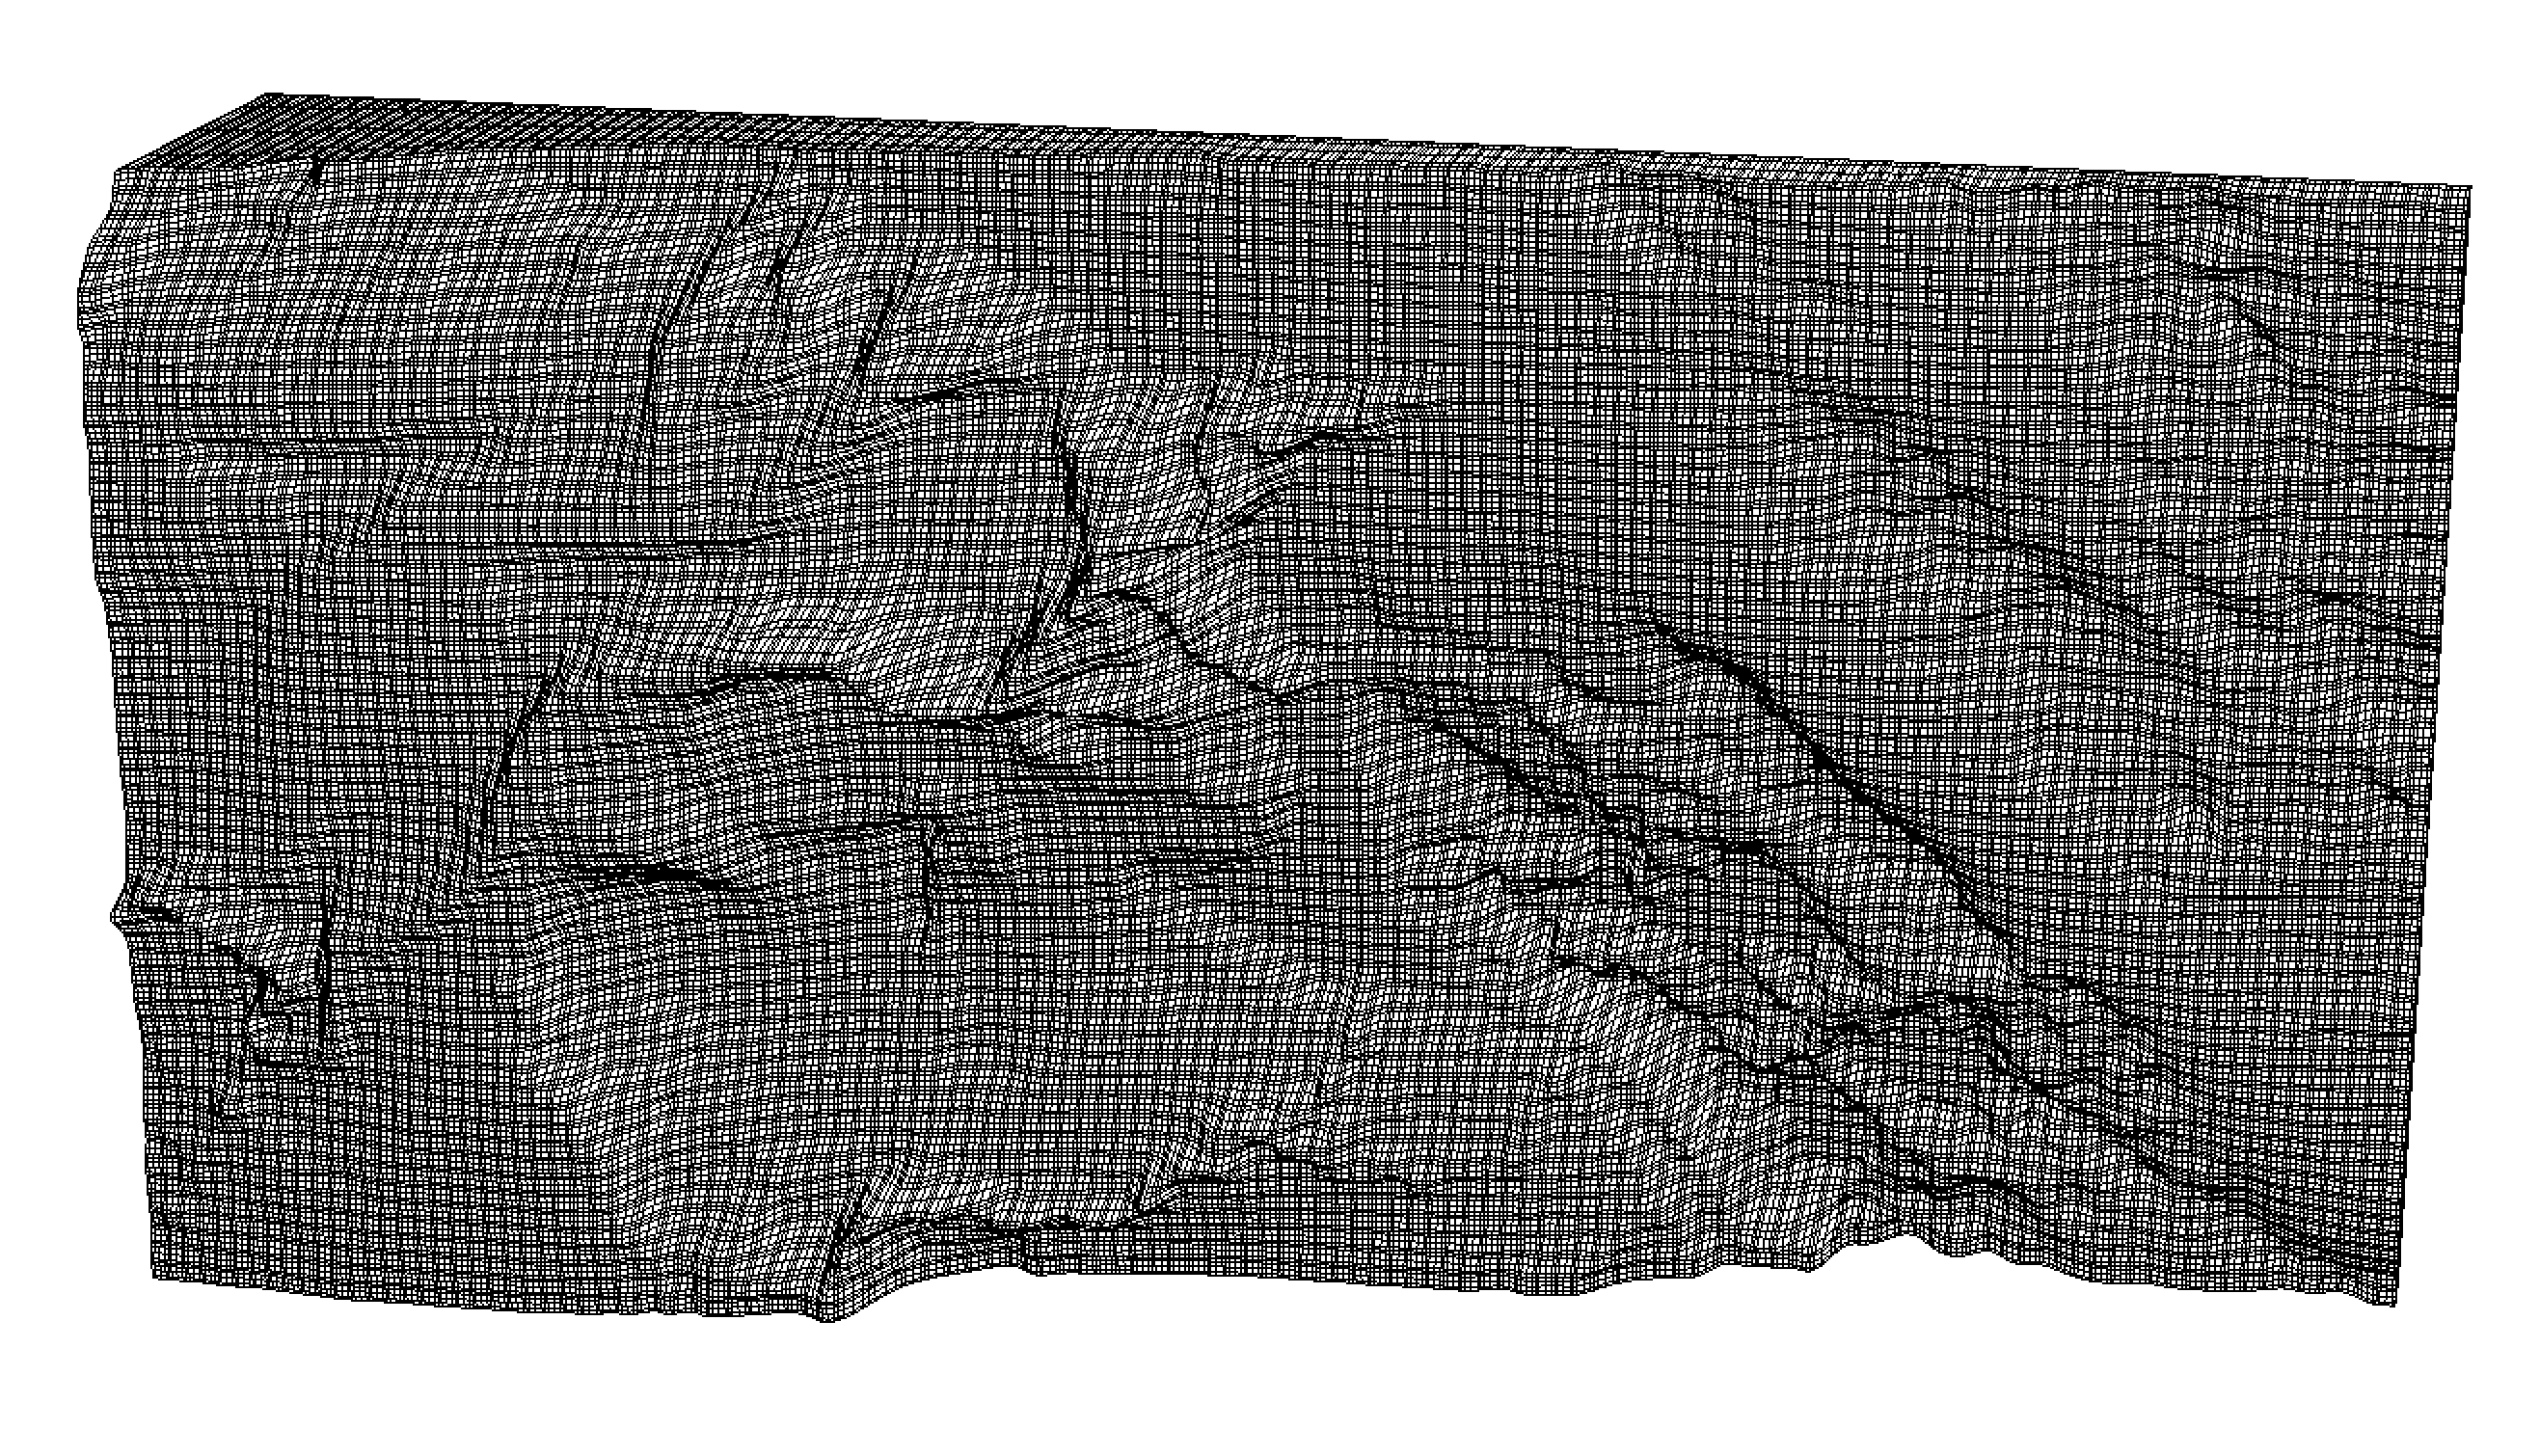
\includegraphics[width=\textwidth]{figures/monterey_with_grid.png}
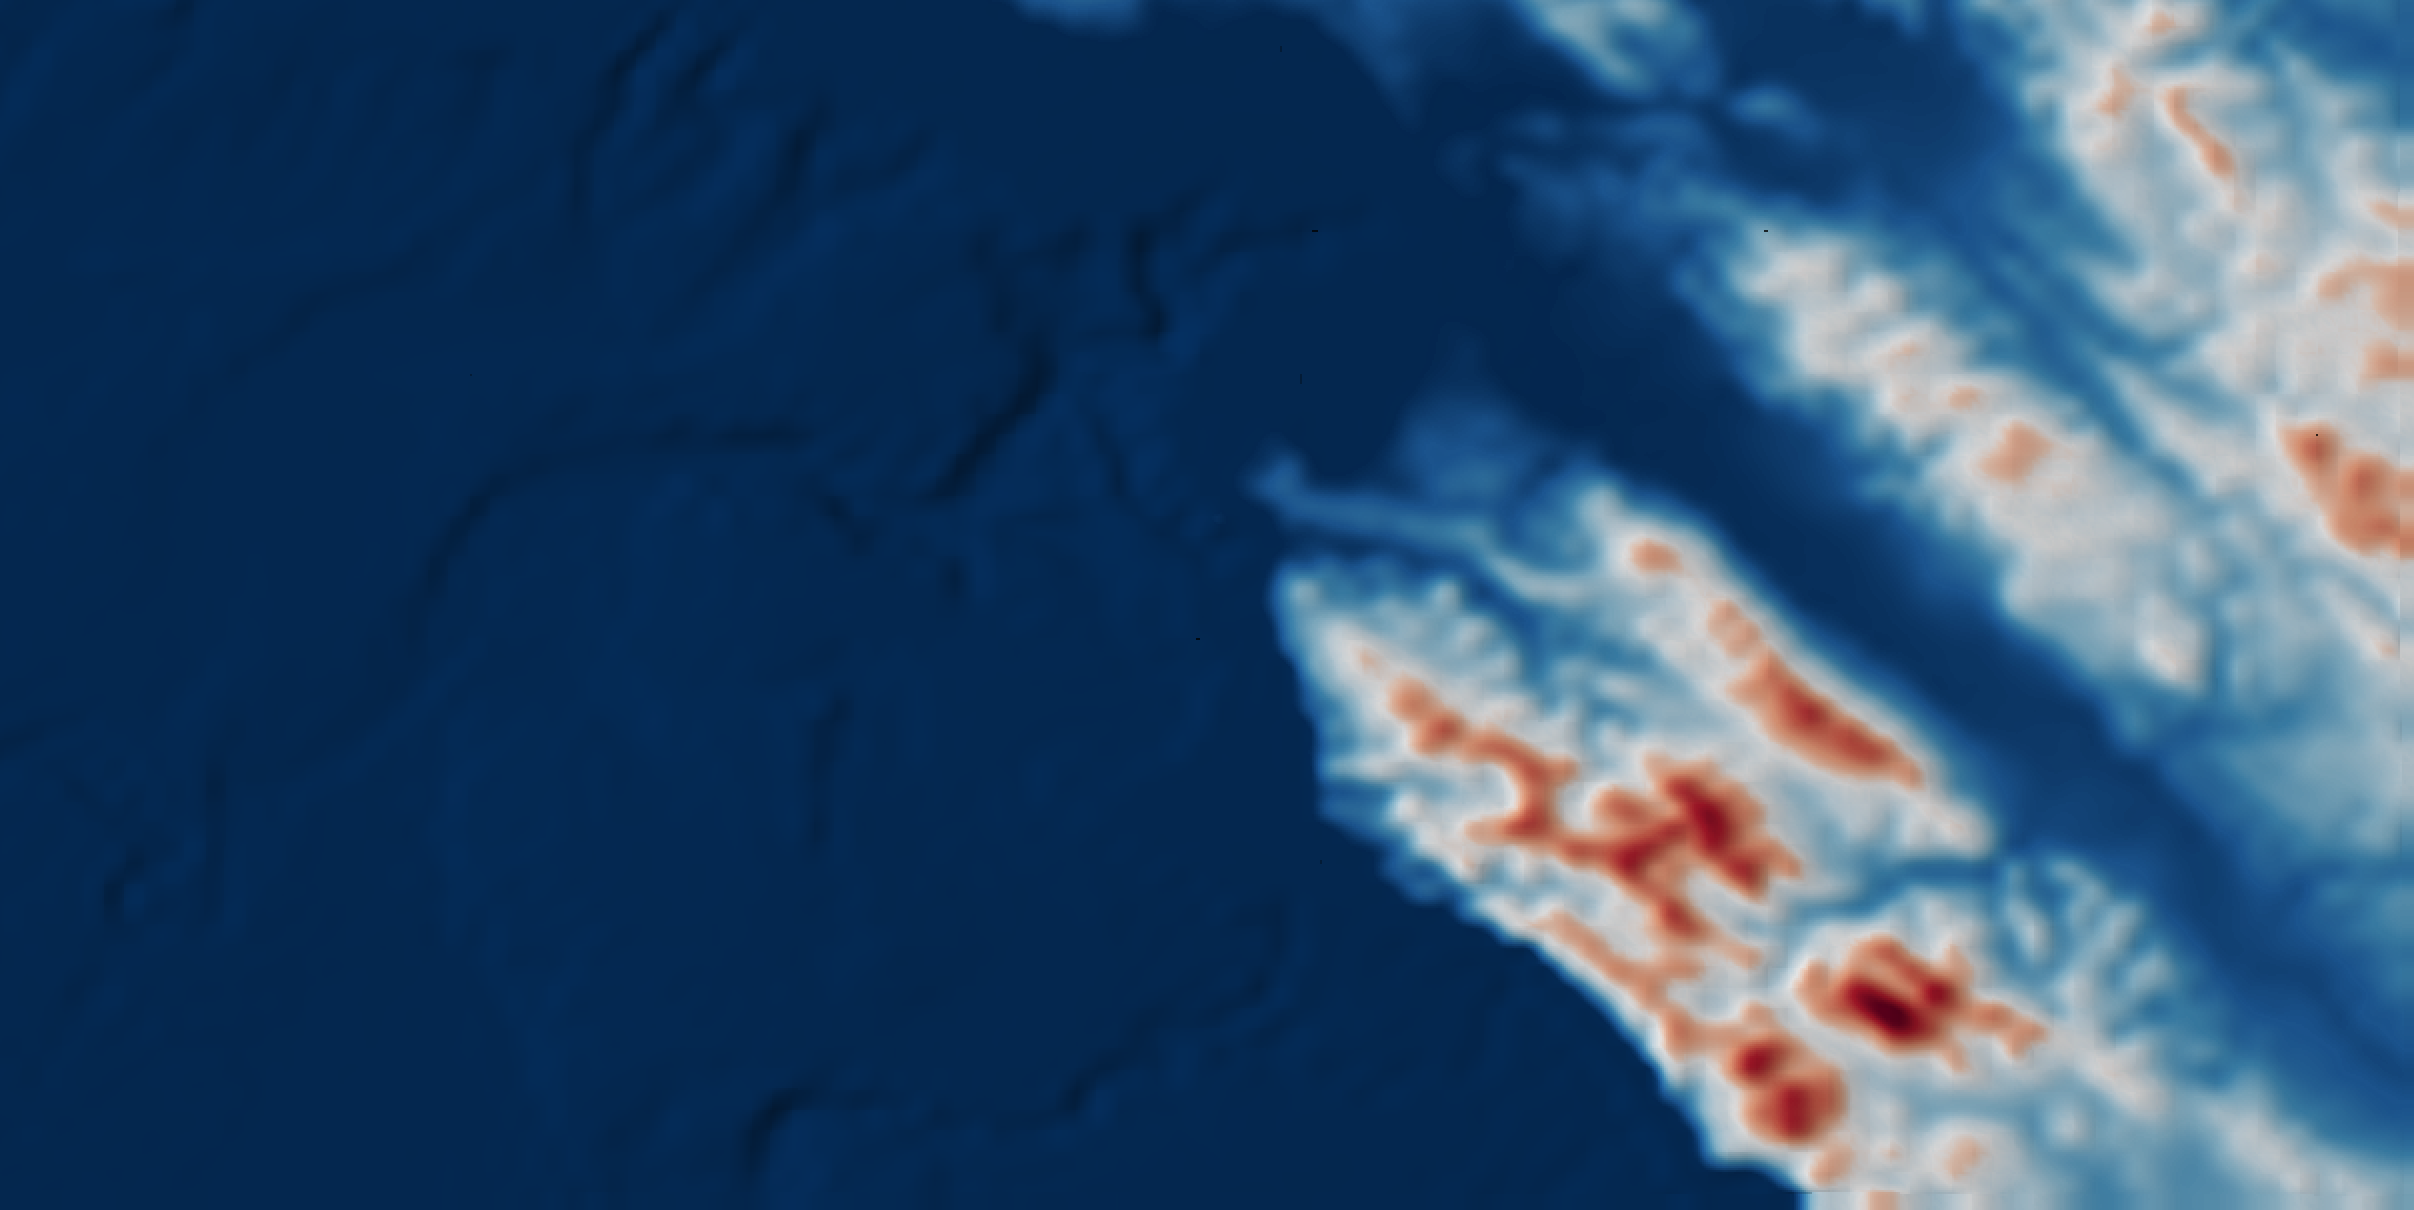
\includegraphics[width=\textwidth]{figures/monterey_colorscale.png}
\caption{Bottom view of the meshed Monterey Bay, California. The high order elements are visible in the top image whereas the topography is colored by its elevation in the bottom.}
\label{fig:montereySurfaceGrid}
\end{figure}

\begin{figure}[htbp]
\centering
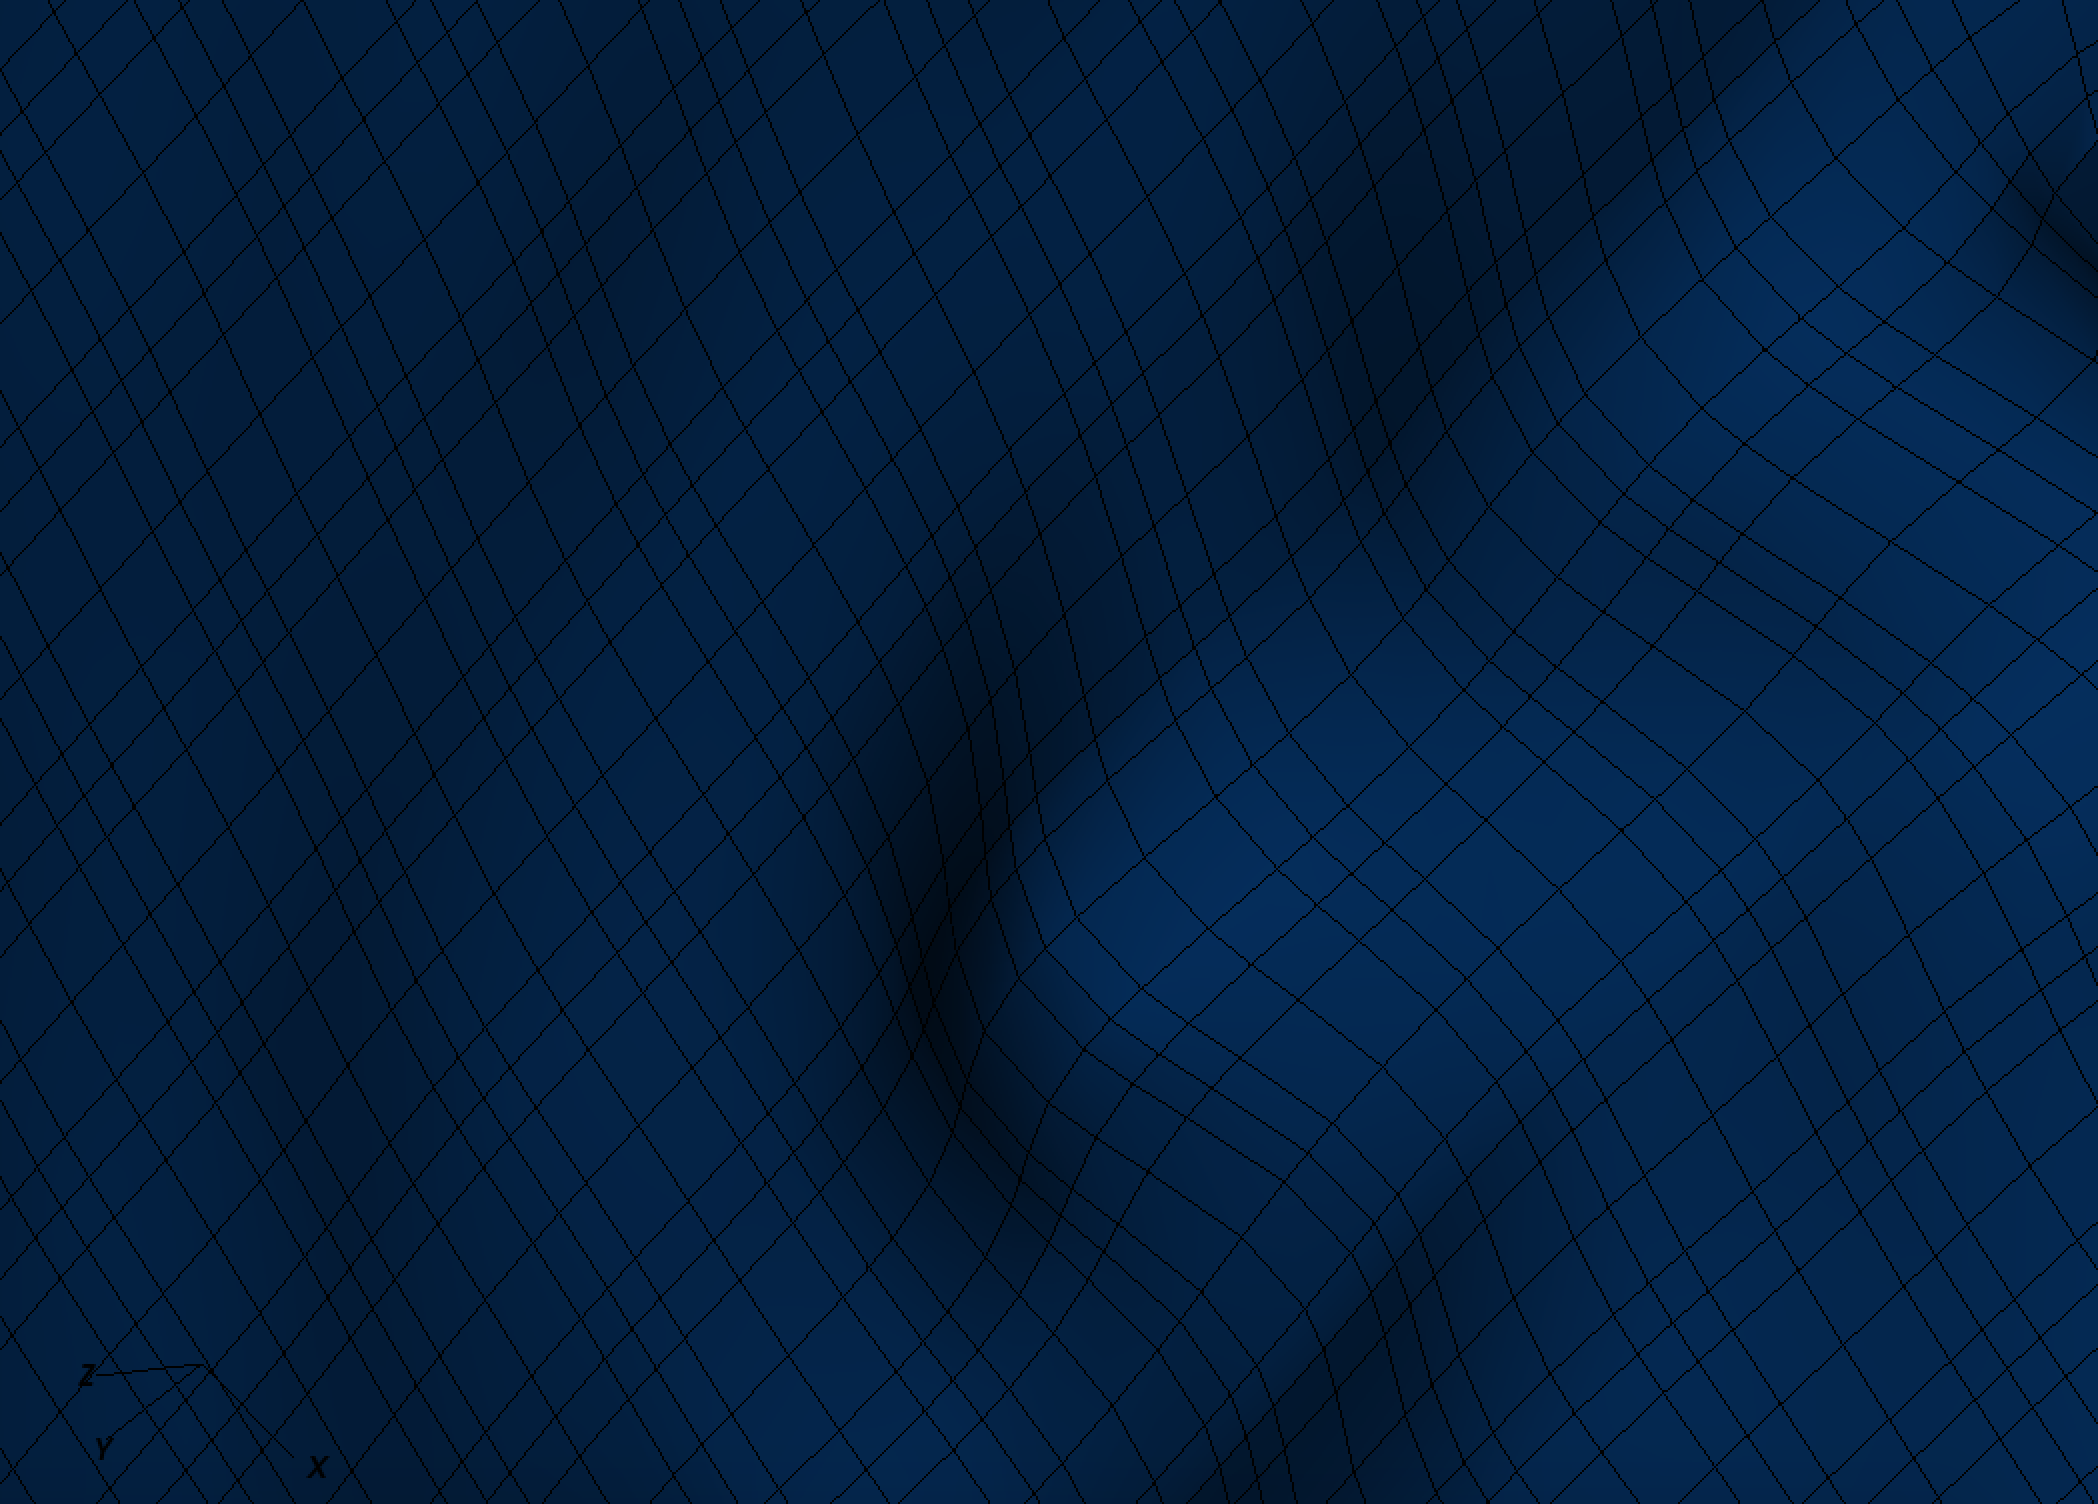
\includegraphics[width=\textwidth]{figures/GRID-detail.png}
\caption{A close view of the curved high order elements on the topography.}
\label{fig:gridDetailView}
\end{figure}

\subsection{Topography/Bathymetry Files and Database}
The external topographic files are not incorporated into the CLIMA repository. 
They are automatically downloaded via a call to {\tt wget} from the {\tt Julia} driver into the user's working directory {\tt \$CLIMA\_HOME/USERS/TEST/DIRECTORY}. As of now, the available topography files are hosted here \url{https://web.njit.edu/~smarras/TopographyFiles} (notice: this directory is not directly accessible from the browser).

\hl{The grid reader should be enhanced to map the grid onto the sphere. As of now, the grid is read and mapped into a closed box only.}


\chapter{Time Discretization}\label{s:timestepping}

The general, compressible equations of motion we use permit a variety of wave modes with different characteristic speeds. Additionally, the equations contain sources that can add stiffness, for example, microphysical processes that occur on timescales of seconds or less.

The equations permit the following wave modes:
\begin{itemize}
    \item Acoustic waves. They have phase speeds around $300~\mathrm{m~s^{-1}}$ in the atmosphere. Density variations and the terms involving pressure in the momentum and energy equations are essential for their existence.
    \item Gravity waves. They have a spectrum of phase speeds. In a deep atmosphere (e.g., in a GCM), the gravest, external mode has phase speed $(gH)^{1/2} \approx 280~\mathrm{m~s^{-1}}$, where $H\approx 8~\mathrm{km}$ is the atmospheric scale height. The gravity term $-\rho \nabla \Phi$ in the momentum equation and the gravitational potential energy $\Phi$ in the energy equation are responsible for their existence.
    \item Inertia-gravity, Rossby waves, and several other wave modes that owe their existence to the Coriolis acceleration $-2\vec{\Omega} \times \rho \vec{u}$. They have smaller phase speeds than the acoustic and external gravity waves.
\end{itemize}
Additional stiffness in the equations arises from:
\begin{itemize}
    \item Falling precipitation, whose fall velocity $w_{p,i}$ can reach $10~\mathrm{m~s^{-1}}$ and thus exceeds typical vertical velocities resolved in GCMs.
    \item Microphysical source terms, for example, in the equations for suspended specific humidities $q_k$; they depend on the precipitation specific humidity $q_{p,i}$, which can change rapidly because precipitate falls rapidly. 
    \item SGS diffusive fluxes, whose effective vertical velocity can exceed that of the resolved velocities.
    \item Other parameterized SGS fluxes, for example, convective updrafts, whose vertical velocities can likewise be large.
\end{itemize}
By contrast, radiation evolves on longer timescales than the dynamical quantities and hence, because it is expensive to evaluate, usually is evolved forward in time with longer timesteps than the dynamical quantities. 

We need a stable and computationally efficient time discretization strategy that allows some state vector components to be subcycled several times per dynamical timestep (e.g., $q_{p,i}$ and convective updrafts) and allows some rapidly evolving source/sink terms (e.g., from microphysics) to be accumulated over the subcycled timesteps. At the same time, it should allow other terms (e.g., radiative energy fluxes) to be evaluated less frequently. In particular, we need a computationally efficient way of handling the physically insignificant acoustic waves.

\section{Decomposition of Time Tendencies}

To circumvent the time-step restriction due to the fast acoustic and gravity waves, using implicit-explicit (IMEX) methods is one option. For the LES model, if the aspect ratio of the horizontal ($\Delta_h$) to vertical ($\Delta_v$) grid spacing is near unity, using fully 3D-IMEX methods may be an option.  For LES models with aspect ratios of grid elements $\Delta_h/\Delta_v > 1$ and for global atmospheric models, which generally have $\Delta_h/\Delta_v \gg 1$, we use 1D-IMEX methods in which the time-integrator is fully explicit in the horizontal direction (HE) and implicit in the vertical direction (so-called HEVI schemes). 

IMEX methods require the solution of one or more linear systems at each time step. The linear system is global in 3D, and this may limit scalability of IMEX methods in a multi-node computational setting. In that case, split-explicit methods may be a more scalable option to deal with the timestep restrictions. For HEVI schemes, the linear solves are restricted to independent atmospheric columns, which are represented on a single compute node (if the domain decomposition is done in the horizontal). So their scalability across nodes is less restricted.

All of these approaches are based on a decomposition of the total tendency $\vec{\mathcal{T}}$ on the right-hand side of Eq.~\eqref{e:eom_compact} into four terms: 
\begin{itemize}
    \item terms to be treated implicitly, labeled by $I$ (the fastest terms);
    \item terms evaluated at the dynamical (advective) timestep, labeled by $d$;
    \item terms to be subcycled $f$ times for each dynamical timestep, labeled by $+f$ (for fast);
    \item terms to be evaluated every $s$ dynamical timesteps, labeled by $-s$ (for slow).
\end{itemize}
This gives
\[
\frac{\partial \vec{Y}}{\partial t} = \Tvector = - \nabla \cdot \Fvector + \vec{\mathcal{S}} = \Tvector_{I} + \Tvector_{d} + \Tvector_{+f} + \Tvector_{-s}.
\]
To obtain a linear problem for the implicit solve, let us linearize the implicit tendency terms $\Tvector_{I}$ by Taylor expansion around a reference state $\vec{Y}_r$,
\begin{equation}\label{e:imex_linearization}
\Tvector_{I}(\vec{Y}) =  \Tvector_I(\vec{Y}_r) + \vec{\mathcal{L}}_I (\vec{Y} - \vec{Y}_r) + \Tvector^N_{I}(\vec{Y}),
\end{equation}
where 
\begin{equation}
    \vec{\mathcal{L}}_I = \left. \frac{\partial\Tvector_I}{\partial\vec{Y}}\right|_{\vec{Y}_r}
\end{equation} 
is the linear component of the tendency operator and $\Tvector^N_{I}(\vec{Y})$ is the nonlinear residual. This then allows us to write the equation of motion \eqref{e:eom_compact} as
\begin{equation}
\label{eq:IMEX}
\frac{\partial\vec{Y}}{\partial t} =  \vec{\mathcal{L}}_I \vec{Y} + \Bigl(\Tvector_I(\vec{Y}_r) - \vec{\mathcal{L}}_I \vec{Y}_r\Bigr) + \Tvector^N_{I}(\vec{Y}) + \Tvector_{d} + \Tvector_{+f} + \Tvector_{-s}.
\end{equation}
Usually, the reference state $\vec{Y}_r$ is chosen so that the tendency of the reference state, $\Tvector_I(\vec{Y}_r)$, and the linear tendency of the reference state, $\vec{\mathcal{L}}_I \vec{Y}_r$, either vanish individually or cancel each other, so that $\Tvector_I(\vec{Y}_r) - \vec{\mathcal{L}}_I \vec{Y}_r=0$. We will justify this in section~\ref{s:IMEX_general}.

\section{Reference State for Linearization}

Solving for the fastest waves implicitly by a linear solve requires linearization of the fastest tendency terms. We generally use reference states characterized by a temperature $T_r(z)$ that may depend on height $z$ but does not depend on horizontal coordinates or time. We enforce hydrostatic balance, and assume the reference state is dry.
%so that the reference state variables are obtained as described in section~\ref{s:initial_conditions} with zero relative humidity ($\mathrm{RH}=0$): the pressure is obtained from \eqref{eq:hydro_pressure}, the density from \eqref{eq:hydro_density}, and the total specific humidity is set to zero, $q_{t,r}=0$.

Because the reference temperature and thus the reference pressure are assumed to be constant in the horizontal, the reference state is assumed at rest, $\vec{u}_r = 0$, consistent with geostrophic balance. Because the reference state is assumed dry, $q_k= 0$ for $k \in \{ t, v, l, i, p\}$ in the reference state.

More sophisticated reference states for linearization are possible, for example, with a latitudinally varying hydrostatically balanced temperature profile, and with a reference velocity in geostrophic and hydrostatic balance with this temperature field. However, we focus on hydrostatic states at rest for now. 
 
 \section{Solving for Acoustic and Gravity Waves Implicitly}
 \label{s:IMEX_general}

Let us lay out in general terms the linearizations for acoustic and gravity waves that underlie IMEX methods in 1D and 3D. The tendency terms responsible for acoustic waves and gravity waves are
 \begin{equation}
 \Tvector_{I}= -\nabla_{1/3} \cdot
 \begin{pmatrix}
 \rho \vec{u} \\
 p \vec{I}_3 \\
 \bigl(e^{\mathrm{tot}} + (\delta_{\mathrm{gw}}-1) \Phi + p/\rho \bigr) \rho \vec{u} \\
 0\\
 \vdots
 \end{pmatrix}
 - \begin{pmatrix}
 0 \\
 \delta_{\mathrm{gw}} \rho \nabla_{1/3} \Phi \\
 0\\
 0\\
 \vdots
 \end{pmatrix},
 \label{eq:3d-imex/tendencies}
 \end{equation}
where all components indicated by dots are zero. The operator $\nabla_{1/3}$ is the 3D differential operator $\nabla_3 = \nabla$ for 3D-IMEX, and it is the 1D operator $\nabla_1 = \vec{k} \partial/\partial_z$ for 1D-IMEX. (The geopotential gradient $\nabla_{1/3} \Phi$ only has a vertical component as long as we consider a spherical planet, so this gradient even in 3D usually only has a vertical component.) The switch $\delta_{\mathrm{gw}}$ (which can only take the value of either $0$ or $1$) is included to indicate whether gravity waves are included in the implicit tendencies: 
\begin{itemize}
    \item $\delta_{\mathrm{gw}}=1$: both acoustic and gravity waves are included in $\Tvector_I$;
    \item $\delta_{\mathrm{gw}}=0$: only acoustic waves are included in $\Tvector_I$.
\end{itemize}

In the tendency \eqref{eq:3d-imex/tendencies}, the terms that need to be linearized are the pressure $p$, which depends nonlinearly on state variables, and the total enthalpy flux $(\rho e^{\mathrm{tot}} + p/\rho) (\rho \vec{u})$. Linearization around a state of rest ($\vec{u}_r=0$) with reference total energy $e^{\mathrm{tot}}_r$, pressure $p_r$, and density $\rho_r$ leads to
 \begin{equation}\label{e:IMEX_linear}
 \vec{\mathcal{L}}_I \vec{Y} = 
 -\nabla_{1/3} \cdot \begin{pmatrix}
 \textcolor{blue}{\rho \vec{u}} \\
 \textcolor{blue}{p_L} \vec{I}_3  \\
 \Bigl(e^{\mathrm{tot}}_r  + (\delta_{\mathrm{gw}}-1)\Phi + p_r/\rho_r \Bigr) \textcolor{blue}{\rho \vec{u}}\\
 0\\
\vdots
\end{pmatrix}
-
\begin{pmatrix}
0 \\
\delta_{\mathrm{gw}} \textcolor{blue} \rho \nabla_{1/3} \Phi \\
0\\
0\\
\vdots
\end{pmatrix}.
\end{equation}
This is linear with respect to \textcolor{blue}{$\rho$} and \textcolor{blue}{$\rho \vec{u}$} (all state variables and linear functions thereof are colored \textcolor{blue}{blue}; all other terms are constants or fixed functions of height $z$). For it to be a linear function of all state variables, the pressure \textcolor{blue}{$p_L$} needs to be expressed as a linear function of state variables. To derive a linear approximation for the pressure, we use the ideal gas law $p = R_m (\rho T)$ and the expression derived from the temperature equation 
%Eq.~\eqref{eq:temperature} 
for $\rho T$ in terms of the internal energy and specific humidities,
\begin{equation}\label{e:pressure}
\begin{split}
p &= R_m (\rho T) \\
  &= \rho R_m T_0 + \frac{R_m}{c_{vm}} \left[\rho e^{\mathrm{tot}} - \rho \Phi - 0.5 \rho \|\vec{u}\|^2 - (\rho q_t - \rho q_l) I_{v,0} + \rho q_i (I_{i,0} + I_{v,0}) \right],
\end{split}
\end{equation}
where we have used the relation $I = e^{\mathrm{tot}} - \Phi - 0.5 \|\vec{u}\|^2$ between total and internal energy. Linearization $p_L = p_r + (\partial p/\partial\vec{Y})\cdot(\vec{Y}-\vec{Y}_r)$ around the reference state $\vec{Y}_r$ with pressure $p_r$ and zero specific humidities leads to 
\begin{equation}\label{eq:pressure_linear}
\textcolor{blue}{p_L} = \textcolor{blue}{\rho} R_d T_0 + \frac{R_d}{c_{vd}} \bigl[ \textcolor{blue}{\rho e^{\mathrm{tot}}} - \textcolor{blue}{\rho} \Phi - (\textcolor{blue}{\rho q_t} - \textcolor{blue}{\rho q_l})I_{v,0} + (\textcolor{blue}{\rho q_i}) (I_{i,0} + I_{v,0}) \bigr].
\end{equation}
If only the total specific humidity $q_t$ is available as a prognostic variable and condensate is determined by saturation adjustment, the condensate specific humidities $q_l$ and $q_i$ in this linearized expression for the pressure can be set to zero. Note that the temperature $T_0$ that appears here is the \emph{reference temperature in the definition of internal energy}, a model constant; it is \emph{not} the temperature $T_r$ of the reference state about which we linearized. In fact, the linearized pressure \eqref{eq:pressure_linear} does not depend on the reference state: the zeroth-order term $p_r$ in the linearization cancels the terms involving the reference state in the linear term, which ensures that the linearized pressure vanishes when the density vanishes. 

We can now see that the sum of the terms involving the reference state in the decomposition \eqref{e:imex_linearization} vanishes,
\[
\Tvector_I(\vec{Y}_r) - \vec{\mathcal{L}}_I \vec{Y}_r = 0.
\]
To see this, it is useful to distinguish the cases when gravity waves are included in the implicit term and when they are not included: 
\begin{itemize}
    \item Acoustic and gravity waves included ($\delta_{\mathrm{gw}}=1$). In this case, it is evident that $\Tvector_I(\vec{Y}_r)=0$ because the pressure gradient ($-\nabla_{1/3} p_r(z)$) and geopotential gradient ($-\rho_r\nabla_{1/3}\Phi$) in the momentum equation (second component of tendency vector) cancel for a hydrostatic reference state with $p_r = p_r(z)$. The same is true for the linear term for a reference state at rest, for which $p_L = p_r$ and $\vec{\mathcal{L}}_I \vec{Y}_r = 0$. 
    \item Only acoustic waves included ($\delta_{\mathrm{gw}}=0$). In this case, neither $\Tvector_I(\vec{Y}_r)$ nor $\vec{\mathcal{L}}_I\vec{Y}_r$ vanish individually, because the geopotential term needed for the cancellation of terms in hydrostatic balance does not appear in the momentum tendency. However, $p_L = p_r$ in a reference state at rest, so that $\Tvector_I(\vec{Y}_r) = \vec{\mathcal{L}}_I\vec{Y}_r$.
\end{itemize}
Thus, in either case, the terms involving the reference state do not appear  in the decomposition \eqref{e:imex_linearization}. 

The nonlinear term follows as the residual 
\begin{equation}\label{e:nonlinear_residual}
\begin{split}
\Tvector^N_{I}(\vec{Y}) & =  \Tvector_I(\vec{Y}) - \vec{\mathcal{L}}_I \vec{Y} \\
& = 
-\nabla_{1/3} \begin{pmatrix}
0 \\
(p - p_L) \vec{I}_3\\
(e^{\mathrm{tot}}  + p/\rho - e^{\mathrm{tot}}_r - p_r/\rho_r) \rho \vec{u}\\
0\\
\vdots
\end{pmatrix}.
\end{split}
\end{equation}
We can verify that the nonlinear residual is small relative to the linear tendency term, as is required for an IMEX approach, as follows. The full pressure (Eq.~\ref{e:pressure}) differs from its linearized counterpart (Eq.~\ref{eq:pressure_linear}) in the inclusion of the kinetic energy term $0.5 \|\vec{u} \|^2$ and of the effects of moisture on the gas constant and specific heat. Relative to the internal energy, the kinetic energy is of order $\|\vec{u}\|^2/c_s^2$ (where $c_s$ is the speed of sound; 
%see section~\ref{s:energy_balance})
and the moisture effects on the gas constant and specific heat are of order $q_t$. Thus, the nonlinear residual $p-p_L$ is small relative to the full pressure $p$: typically of order $10^{-3}$ in Earth's atmosphere. The nonlinear residual in the energy equation depends on the choice of reference state. With a reference temperature $T_r(z)$ that depends on height $z$ only, one may expect $T - T(z) \lesssim 30~\mathrm{K}$ in Earth's atmosphere. Because the internal energy deviation from the reference state dominates the residual $e^{\mathrm{tot}} - e^{\mathrm{tot}}_r$, one may expect a size of the residual $e^{\mathrm{tot}} - e^{\mathrm{tot}}_r$ relative to the full total energy $e^{\mathrm{tot}}$ of order $30~\mathrm{K}/300~\mathrm{K} = 10^{-1}$. Hence, the nonlinear residual in the energy equation is likewise small compared with the linear tendency term. 
 
The decomposition of $\Tvector_I$ up to this point is general and holds for 3D-IMEX and 1D-IMEX, with the appropriate differential operator substituted for $\nabla_{1/3}$.

\subsection{3D IMEX}

For 3D IMEX, $\nabla_{3} = \nabla$. The only nonzero linear tendencies in Eq.~\eqref{e:IMEX_linear} are those for 
\begin{enumerate}
    \item Density $\rho$,
    \item Three velocity components $\vec{u}$,
    \item Energy $e^{\mathrm{tot}}$,
\end{enumerate}
that is, for 5 scalars. All other scalars (e.g., specific humidity variables) do not enter the implicit linear solve. 

\subsection{1D IMEX}

For 1D IMEX, $\nabla_{3} = \vec{k} \partial/\partial z$. The only nonzero linear tendencies in Eq.~\eqref{e:IMEX_linear} are those for 
\begin{enumerate}
    \item Density $\rho$,
    \item The vertical velocity component $w = \vec{k} \cdot \vec{u}$,
    \item Energy $e^{\mathrm{tot}}$,
\end{enumerate}
that is, for 3 scalars. The linear tendencies of the horizontal velocity components vanish. Hence, these do not enter the implicit linear solve, and neither do other scalars. 

\section{Additive Runge-Kutta IMEX Methods}

We use a general family of additive Runge-Kutta methods (ARK) methods for 1D and 3D IMEX approaches \citep[see, e.g.,][]{giraldo:2013,Weller13a,Gardner18a}. The same infrastructure of the linear (implicit) and nonlinear (explicit) decomposition can also be used in substepping (e.g., split-explicit or multirate) approaches.

\hl{[We need this to be formulated generally, for 3D or 1D IMEX. This means restricting the linear solves to the relevant subset of state variables. Make this clear in the notation so it can be implemented. Also make clear which of these algorithms we should prioritize.]}

Assuming that $\Tvector_I(\vec{Y}_r) - \vec{\mathcal{L}}_I \vec{Y}_r=0$, let us
rewrite Eq.~\eqref{eq:IMEX} as
\begin{equation}
\label{eq:IMEX_v3}
\frac{\partial\vec{Y}}{\partial t} =  \vec{\mathcal{L}}_I \vec{Y} + \Tvector_{d'} + \Tvector_{-s} + \Tvector_{+f}
\end{equation}
where $\Tvector_{d'}=\Tvector^N_{I} + \Tvector_{d}$ captures the sum of the dynamical tendencies and the nonlinear remainder tendencies after the linear implicit tendencies are taken into account.  

If for now we neglect $\Tvector_{+f}$ (e.g., view it as included in  $\Tvector_{d'}$), a first 3D-IMEX algorithm with superstepping of the slow tendencies takes the following form:
\begin{algorithm}
\label{alg:3d-imex_v1}
\begin{algorithmic}
\State
\Function{3D-IMEX with Superstepping}{}
\For{$i=1:S$} 
\State $\left( \vec{I} - \Delta t \widetilde{a}_{ii} \vec{\mathcal{L}}_I \right) \vec{Y}^{(i)}=\vec{Y}^{n} + \Delta t \sum_{j=1}^{i-1} \left( a_{ij} \Tvector_{d'}(\vec{Y}^{(j)}) + a_{ij} \Tvector_{-s}(\red{\vec{Y}^{n-s}})
+ \widetilde{a}_{ij} \vec{\mathcal{L}}_I \vec{Y}^{(j)} \right)$ 
\EndFor %i
\State $\vec{Y}^{n+1}=\vec{Y}^{n} + \Delta t \sum_{i=1}^{S} b_{i} \left[ \Tvector_{d'}(\vec{Y}^{(i)}) + \Tvector_{-s}(\red{\vec{Y}^{n-s}})
+ \vec{\mathcal{L}}_I \vec{Y}^{(i)} \right]$
\EndFunction
\end{algorithmic}
\end{algorithm}
In Alg.\ \ref{alg:3d-imex_v1}, the fastest waves (e.g., acoustic and gravity waves) are solved implicitly for each stage $i$ of the RK method with $S$-stages. The term $\red{\vec{Y}^{n-s}}$ is frozen at the time level $n-s$, and $a_{ij}$, $\widetilde{a}_{ij}$; and $b_i$ are the RK coefficients in Butcher tableau form (see Table \ref{eq:butcher_tableau}).
\begin{equation}
\begin{array}{c|c}
\ST c&A\\
\hline
\ST  & b\transpose
\end{array}
\hspace{0.5in}
\begin{array}{c|c}
\ST \wt{c} & \wt{A} \\
\hline
\ST  & \wt{b} \transpose
\end{array}
\label{eq:butcher_tableau}
\end{equation}
Here, $A=a_{ij}, \; i,j=1,\ldots S$, and $c_i=\sum_{j} a_{ij}$ represent the time when the right-hand side is evaluated; that is, we evaluate it at each stage which occurs at the time interval $t+c_i \dt$.
In addition, $b=\wt{b}$ is necessary in order to conserve all linear invariants \citep{giraldo:2013}. If we now include the fast terms denoted by $\Tvector_{+f}$ then we can modify Alg.\ \ref{alg:3d-imex_v1} as summarized in Alg.\ \ref{alg:3d-imex_v2}, where for simplicity we assume a 3-partition IMEX multirate strategy based on Euler's method.
\begin{algorithm}
\label{alg:3d-imex_v2}
\begin{algorithmic}
\State
\Function{3D-IMEX Multirate with 3-Partitions based on Euler's Method}{}
\State $\vec{Y}^{(0)}=\vec{Y}^{n}$
\For{$m=1:M$} 
\State $\vec{Y}^{(m)}=\vec{Y}^{(m-1)} + \frac{\Delta t}{M} \Tvector_{+f}(\vec{Y}^{(m)})$
\EndFor %m
\State $\left( \vec{I} - \Delta t \vec{\mathcal{L}}_I \right) \vec{Y}^{(M)}=\vec{Y}^{(m)}$
\State $\vec{Y}^{n+1}=\vec{Y}^{n} + \Delta t \left[ \Tvector_{-s}(\red{\vec{Y}^{n-s}}) + \Tvector_{d'}(\vec{Y}^{(M)}) + 
\Tvector_{+f}(\vec{Y}^{(M)}) + 
\vec{\mathcal{L}}_I \vec{Y}^{(M)} \right]$
\EndFunction
\end{algorithmic}
\end{algorithm}
A more general form of Alg.\ \ref{alg:3d-imex_v2} can be found in Alg.\ \ref{alg:3d-imex_v3}, where we now replace the outside Euler loop with an I-stage Additive Runge-Kutta method. 
\begin{algorithm}
\label{alg:3d-imex_v3}
\begin{algorithmic}
\State
\Function{3D-IMEX Multirate with 3-Partitions based on ARK and Euler's Method}{}
\State $\vec{Y}^{(i)}=\vec{Y}^{n}$
\For{$i=2:I$} 
\State $\vec{Y}^{(0)}=\vec{Y}^{(i)}$
\For{$m=1:M$} 
\State $\vec{Y}^{(m)}=\vec{Y}^{(m-1)} + \frac{\left(c_i - c_{i-1} \right) \Delta t}{M} \Tvector_{+f}(\vec{Y}^{(m)})$
\EndFor %m
\State $\left( \vec{I} - \Delta t \widetilde{a}_{ii} \vec{\mathcal{L}}_I \right) \vec{Y}^{(i)}=\vec{Y}^{(m)} + \Delta t \sum_{j=1}^{i-1} \left( a_{ij} \Tvector_{d'}(\vec{Y}^{(j)}) + \widetilde{a}_{ij} \vec{\mathcal{L}}_I \vec{Y}^{(j)} \right)$
\EndFor %i
\State $\vec{Y}^{n+1}=\vec{Y}^{n} + \Delta t \sum_{j=1}^{i} b_i \left[ \Tvector_{-s}(\red{\vec{Y}^{n-s}}) + \Tvector_{d'}(\vec{Y}^{(i)}) + 
\Tvector_{+f}(\vec{Y}^{(i)}) + 
\vec{\mathcal{L}}_I \vec{Y}^{(i)} \right]$
\EndFunction
\end{algorithmic}
\end{algorithm}

A slightly more general form of Alg.\ \ref{alg:3d-imex_v3} can be found in Alg.\ \ref{alg:3d-imex_v4} where we now replace the inner Euler loop with an J-stage explicit Runge-Kutta method. 
\begin{algorithm}
\label{alg:3d-imex_v4}
\begin{algorithmic}
\State
\Function{3D-IMEX Multirate with 3-Partitions based on ARK}{}
\State $\vec{Y}_i^{(i)}=\vec{Y}^{n}$
\For{$i=2:I$} 
\State $\vec{Y}_j^{(1)}=\vec{Y}_i^{(i)}$
\For{$j=2:J$} 
\State $\vec{Y}_j^{(j)}=\vec{Y}_i^{(i-1)} + \left(c_i - c_{i-1} \right) \Delta t \sum_{k=1}^{j-1} a_{jk} \Tvector_{+f}(\vec{Y}_j^{(k)})$
\EndFor %j
\State $\vec{Y}^{(*)}=\vec{Y}_i^{(i-1)} + \left(c_i - c_{i-1} \right) \Delta t \sum_{j=1}^{J} b_j \Tvector_{+f}(\vec{Y}_j^{(j)})$
\State $\left( \vec{I} - \Delta t \widetilde{a}_{ii} \vec{\mathcal{L}}_I \right) \vec{Y}_i^{(i)}=\vec{Y}^{(*)} + \Delta t \sum_{j=1}^{i-1} \left( a_{ij} \Tvector_{d'}(\vec{Y}_i^{(j)}) + \widetilde{a}_{ij} \vec{\mathcal{L}}_I \vec{Y}_i^{(j)} \right)$
\EndFor %i
\State $\vec{Y}^{n+1}=\vec{Y}^{n} + \Delta t \sum_{i=1}^{I} b_i \left[ \Tvector_{-s}(\red{\vec{Y}^{n-s}}) + \Tvector_{d'}(\vec{Y}_i^{(i)}) + 
\Tvector_{+f}(\vec{Y}_i^{(i)}) + 
\vec{\mathcal{L}}_I \vec{Y}_i^{(i)} \right]$
\EndFunction
\end{algorithmic}
\end{algorithm}
A challenge in implementing Alg.\ \ref{alg:3d-imex_v4} is that we require two stage value storages: one for the $i$-loop and the other for the $j$-loop, which have different Butcher tableaux and store the solution at different times in the interval $[t^n,t^{n+1}]$.
[\fxg{To do: add an interior m-loop for subcycling. This section will be compressed once  I get the general form worked out.}]

For any of these 3D IMEX time stepping strategies, the maximum eigenvalue of the Jacobian operators is $\lambda_{I}=\widehat{\vec{n}} \cdot \vec{u} + c_{s}$ \hl{[define $\widehat{\vec{n}}$, seems to be elementwise, and differing in use from spatial discretization section]} (corresponding to $\Tvector_{I}$) and  $\lambda^L_{I} = c^L_s$ (corresponding to $\vec{\mathcal{L}}_{I}\vec{Y}$), where $c_s$ is the speed of sound and $c^L_s$ is the speed of sound in the reference state. %The speed of sound can be approximated by the expression \eqref{e:soundspeed}, which neglects (small) modifications of sound speed from the stratification of the background state \citep{Durran99}.

\comment{
\begin{algorithm}
\label{alg:3d-imex_v2}
\begin{algorithmic}
\State
\Function{3D-IMEX with Substepping}{}
\For{$i=1:Stages$} 
\State $\left( \vec{I} - \Delta t \widetilde{a}_{i,i} \vec{\mathcal{L}}_I \right) \vec{Y}^{(i)}=\vec{Y}^{n} + \Delta t \sum_{j=1}^{i-1} \left( a_{i,j} \Tvector_{d'}(\vec{Y}^{(j)}) + a_{i,j} \Tvector_{-s}(\vec{Y}^{n-s})
+ \widetilde{a}_{i,j} \vec{\mathcal{L}}_I \vec{Y}^{(j)} \right)$ 
\For{$m=1:M_{steps}$}
\State $\vec{Y}^{(m)} = \vec{Y}^{(i)} + \Delta \tau \Tvector_{+f} (\vec{Y}^{(m)} )$ \Comment \fxg{simple Euler substepping with time-splitting (large splitting errors)}
\EndFor %m
\State $\vec{Y}^{(i)} = \vec{Y}^{(m)}$
\EndFor %i
\State $\vec{Y}^{n+1}=\vec{Y}^{n} + \Delta t \sum_{i=1}^{Stages} b_{i} \left( \Tvector_{d'}(\vec{Y}^{(i)}) 
+ \vec{\mathcal{L}}_I \vec{Y}^{(i)} \right)$
\EndFunction
\end{algorithmic}
\end{algorithm}
In Alg.\ \ref{alg:3d-imex_v2}, $\Delta \tau=\frac{\Delta t c_i}{M_{steps}}$ where $c_i=\sum_{j=1}^{i-1} a_{i,j}$.
Note that in Alg.\ \ref{alg:3d-imex_v2}, the $m$-loop can be replaced by another RK loop with stage-order greater than or equal to $S$. If the stage-order of this loop is chosen to be $S$ then we can effectively increase the stability of the method by a factor of 2 with respect to time-step (this means that the terms in $\Tvector_{+f}$ can be twice as fast as those in $\Tvector_{d'}$.
[\fxg{In progress. Need to know what is in $\Tvector_{+f}$ in order to see how to fractional-step or substep properly and accurately.  E.g., are these entirely separate processes or do they contain the prognostic variables that we have in the other operators.}] \hl{[TS: The most important case is where the fast explicit tendencies contain the horizontal sound and gravity waves; that is, the vertical components are solved for implicitly, but the horizontal components are advanced with explicit substeps. So it's the horizontal components of the same tendency terms whose vertical components are included in the implicit solve.]}}

\comment{
To discretize the equations in time using an ARK method, we first compute the stage values \hl{\textbf{Frank}: This subsection below here needs work. A number of things are unclear/incorrect/} [\fxg{Yes, unclear and incorrect. However, some of what is here I did not write. Let me try to fix this after the substepping.}]
\begin{multline}\label{eq:IMEX/stages}
\statestage^{(i)}= \vec{Y}^n + \Delta t \sum_{j=0}^{i} \left( a^{I}_{ij} \vec{\mathcal{L}}_{I} \statestage^{(j)} \right) + \Delta t \sum_{j=0}^{i-1} \left( {a}^{+f}_{ij} \Tvector_{+f}(\statestage^{(j)}) \right)  \\
+  \Delta t \sum_{j=0}^{i-1} \left( {a}^{d}_{ij} \bigl(\Tvector_{d}(\statestage^{(j)}) + \Tvector^N_I(\statestage^{(j)})\bigr)\right) \\
+ \Delta t \sum_{j=0}^{i-1} \left( {a}^{-s}_{ij} \Tvector_{-s}(\statestage^{(j)}) \right) + \Delta t \Bigl(\Tvector_I(\vec{Y}_r) - \vec{\mathcal{L}}_I \vec{Y}_r \Bigr) \sum_{j=0}^i a_{ij}^I 
\end{multline}
where $i=1,\ldots,s$ labels the $s$ stages, and $\statestage^{(0)}=\vec{Y}^n$ (where $\vec{Y}^n$ is the solution vector at the current time). The coefficients $a$ are the coefficients of the partitioned Butcher tableau (see, e.g., \citet{constantinescu:2007, constantinescu:2010c}). Here, the nonlinear residual of the implicit term was assumed to evolve with other terms on dynamical timescales. Some rows of the coefficient matrices $a$ for the slower component will be zero. \hl{Make the subcycling explicit. We need to see where computational gains come from. Can we write this out explicitly now, even without having the Butcher tableaus worked out?} 
The solution at time $n+1$ is obtained from
\be
\vec{Y}^{n+1}=\vec{Y}^n + \Delta t \sum_{i=0}^{s} \left( b_i \vec{\mathcal{T}}(\statestage^{(i)}) \right).
\label{eq:IMEX/update}
\ee
\hl{[Really? It seems odd to have the same set of weights $b$ for all tendency terms. The sub- and supercycling should be manifest here.]} 
We are restricting ourselves to diagonally-implicit Runge-Kutta (DIRK) methods for which $a^I_{ij} = 0$ for $i>j$ \hl{[]Is this ok? That is, apply this condition just for implicit coefficients?]} \citep{alexander:1977,butcher:1981a,ascher:1997,boscarino:2009}.  To make the DIRK more efficient, we additionally impose the restriction that all diagonal values ${a}^I_{ii}$ are the same \hl{[ok? just for implicit components?]} This allows one construction of the matrix problem for the implicit solve that does not change across stage values. We refer to this as singly-diagonally-implicit Runge-Kutta (SDIRK).

Rearranging Eq.~\eqref{eq:IMEX/stages} as follows 
\begin{multline}\label{eq:IMEX/stages2}
\left( \vec{I} - {a}^{I}_{ii}\vec{\mathcal{L}}_{I} \right)  \statestage^{(i)}  =  \vec{Y}^n + 
\Delta t \sum_{j=0}^{i-1} \left( {a}^{+f}_{ij} \Tvector_{+f}(\statestage^{(j)}) \right)   \\
+ \Delta t \sum_{j=0}^{i-1} \left( {a}^{d}_{ij} \bigl(\Tvector_{d}(\statestage^{(j)}) + \Tvector^N_I(\statestage^{(j)})\bigr) \right) \\
+ \Delta t \sum_{j=0}^{i-1} \left( {a}^{-s}_{ij} \Tvector_{-s}(\statestage^{(j)}) \right) + \Delta t \bigl(\Tvector_I(\vec{Y}_r) - \vec{\mathcal{L}}_I \vec{Y}_r \bigr) \sum_{j=0}^i a_{ij}^I
\end{multline}
reveals the implicit nature of the problem. Letting $\vec{A}=\vec{I} - {a}^{I}_{ii} \vec{\mathcal{L}}_{I}$, $\vec{X}=\statestage^{(i)}$, and denoting the right-hand side of Eq.~\eqref{eq:IMEX/stages2} by $\mathcal{B}$, we obtain the linear system 
\[
\vec{A} \vec{X} = \mathcal{B}.
\]
We can solve this linear system using, e.g., Krylov subspace methods such as GCR or GMRES (we cannot use conjugate gradient since the system is hyperbolic and therefore is not symmetric positive-definite in the current form). ARK of order $\order(\Delta ^k)$ for $k=2,\ldots,5$ are planned (which are roughly of order $k=s-1$ where $s$ denotes the number of stages.
}


\comment{
\section{3D-IMEX Approach: Version 2}
\label{sec:3D-IMEX/v2}
The advantage of using version 1 presented in Sec.\ \ref{sec:3D-IMEX/v1} is that we can construct the explicit solution of the governing equations and then view the implicit portion of the IMEX method as a correction to the explicit solution.  However, following this approach may cause the discrete form of the equations to lose hyperbolicity (see \cite{bispen:2017}).

To avoid this situation, we split the $\vec{\mathcal{T}}$ operator directly into a linear and nonlinear part:
\begin{equation}
 \vec{\mathcal{T}}(\vec{Y})=- \left( \begin{array}{c}
 0 \\
 \nabla \cdot (\rho \vec{u} \otimes \vec{u}) \\
 \nabla \cdot ( (E' + p') \vec{u} )
\end{array}
\right) 
+
\left( \begin{array}{c}
 \nabla \cdot (\rho \vec{u} ) \\
 \nabla p'  + \rho' \nabla \Phi \\
 \nabla \cdot ( (E_r + p_r) \vec{u} )
\end{array}
\right).
\label{eq:3d-IMEX/S_operator/split}
\end{equation}
 Here, we have eliminated the reference pressure gradient and reference buoyancy due to, e.g., hydrostatic balance. With this approach, the maximum eigenvalue for the Jacobian operators are $\lambda^{(N)}_{\max}=2 \widehat{\vec{n}} \cdot \vec{u}$ and 
 $\lambda^{(L)}_{\max}= c_s$, where the superscripts (N) and (L) denote the operator that the eigenvalue is associated with.
}

% \subsubsection{3D-IMEX Linear Operator in the Reference Coordinate}
%  Although not strictly necessary to understand the application of the 3D-IMEX approach given by Eqs.\ \eqref{eq:3d-imex/linear_operator} and \eqref{eq:3d-imex/linear_fluxes} let us describe the approximation of the spatial derivatives in terms of the reference element coordinates; note that this will assist us in understanding the 1D-IMEX approach described below. Let us first rewrite the 3D-IMEX linear operator 
%  $\Tvector_{I}$ as follows:
%  \begin{equation}
%  \Tvector_{I}= \nabla \cdot \left( \begin{array}{c}
%  \rho \vec{u} \\
%  p' \vec{I}_3 \\
%  \left( e_r + \frac{p_r}{\rho_r} \right) \rho \vec{u} \\
% \vec{0}\\
% \vec{0} \\
% \vec{0}
% \end{array}
% \right), 
% \label{eq:3d-imex/linear_operator_v2}
% \end{equation}
%  where we can now replace the differential operator $\nabla=\diff{}{x_1} \hat{\vec{x}}_1 + \diff{}{x_2} \hat{\vec{x}}_2 + \diff{}{x_3} \hat{\vec{x}}_3$
%  by the following
%  \[
%  \nabla \cdot \vec{f} = \frac{1}{J} \nabla_{\vec{\xi}} \cdot \left(J \vec{f}^{\vec{\xi}} \right)
%  \]
%  where $\vec{f}=f_{x_1} \hat{\vec{x}}_1 + f_{x_2} \hat{\vec{x}}_2 + f_{x_3} \hat{\vec{x}}_3$ denotes the (covariant) vector in the model coordinate system, 
%  $\vec{f}^{\vec{\xi}}=f^{\xi_1} \hat{\vec{\xi}}_1 + f^{\xi_2} \hat{\vec{\xi}}_2 + f^{\xi_3} \hat{\vec{\xi}}_3$ denotes the (contravariant) vector in the element reference coordinate system with the components defined as follows:
%  $\vec{f}^{\xi_i}=\vec{f} \cdot \nabla \xi_i$, where $J$ is the determinant of the map Jacobian, and 
%  $\nabla_{\vec{\xi}}=\diff{}{\xi_1} \hat{\vec{\xi}}_1 + \diff{}{\xi_2} \hat{\vec{\xi}}_2 + \diff{}{\xi_3} \hat{\vec{\xi}}_3$. The covariant vector $\vec{f}$ can now take the place of any of the rows in Eq.\ \eqref{eq:3d-imex/linear_operator_v2}.
 
% \section{1D-IMEX Approach}
% \label{sec:1D-IMEX}

% For grid aspect ratios $\Delta_h/\Delta_v \gg 1$, the stiffness of the equations arises principally from vertically propagating sound and gravity waves; vertical diffusion terms may also add stiffness. For this situation, we only need to extract fast terms along the vertical direction and treat them implicitly.  Following the general approach outlined in section~\ref{s:IMEX_general}, using $\delta_{\mathrm{gw}}=1$ to extract sound and gravity waves. (We treat diffusion terms explicitly for the moment.) The linear tendency component $\vec{\mathcal{L}}_I \vec{Y}$ and the nonlinear residual $\Tvector_I^N(\vec{Y})$ are then given by Eqs.~\eqref{e:IMEX_linear} and \eqref{e:nonlinear_residual}, with the derivative operator $\nabla_{1/3} = \vec{k} \partial/\partial z$.

% \subsubsection{1D-IMEX Linear Operator in the Reference Coordinate}
%  Although Eqs. \eqref{eq:1d-imex/linear_operator} -  \eqref{eq:1d-imex/linear_sources} are written with respect to the z-coordinate (direction along which gravity acts) it does not necessarily mean that the model spatial coordinates are aligned in such a fashion (e.g., unless spherical coordinates are used). However, we can construct the grids of the model in a stacked approach such that one reference coordinate is indeed aligned along the z-coordinate. 
%  Replacing the divergence operator acting on a (covariant) vector $\vec{f}$ as follows
%  \[
%  \nabla \cdot \vec{f} = \frac{1}{J} \nabla_{\vec{\xi}} \cdot \left(J \vec{f}^{\vec{\xi}} \right)
%  \]
%  where $\vec{f}^{\vec{\xi}}=f^{\xi_1} \hat{\vec{\xi}}_1 + f^{\xi_2} \hat{\vec{\xi}}_2 + f^{\xi_3} \hat{\vec{\xi}}_3$ denotes the (contravariant) vector in the element reference coordinate system with components defined as follows:
%  $\vec{f}^{\xi_i}=\vec{f} \cdot \nabla \xi_i$, where $J$ is the determinant of the map Jacobian, and 
%  $\nabla_{\vec{\xi}}=\diff{}{\xi_1} \hat{\vec{\xi}}_1 + \diff{}{\xi_2} \hat{\vec{\xi}}_2 + \diff{}{\xi_3} \hat{\vec{\xi}}_3$. 
 
%  Let us rewrite Eqs.\ \eqref{eq:1d-imex/linear_operator}-\eqref{eq:1d-imex/linear_sources} as follows
%  \begin{equation}
%  \mathcal{T}^{3D}_{I} = \nabla \cdot \left( \begin{array}{c}
%  \left( \rho \vec{u} \right) \\
%  p'  \\
%  \left( e_r + \frac{p_r}{\rho_r} \right) \rho \vec{u} \\
%  0 \\
% 0 \\
% 0
% \end{array}
% \right)
% +
% \left( \begin{array}{c}
% 0 \\
% \rho' \nabla \Phi \\
% 0 \\
% 0 \\
% 0 \\
% 0 
% \end{array}
% \right),
% \label{eq:1d-imex/linear_operator_3d}
% \end{equation}
% where we are now considering the fastest waves linear operator in three-dimensional space.
% [\fxg{To Do: separate in terms of reference coordinate to isolate the radial coordinate}]

% \hl{[Important points to keep in mind here: (1) For a global model, we usually use domain decompositions that leave atmospheric columns on one node. This means there is no sizable inter-node communication overhead for 1D-IMEX. The problem for 3D IMEX is that the linear solve can involve states distributed across nodes, and hence involves inter-node communication. This may not scale well, and split-explicit schemes may be preferable in that case. We need to test to find out. We should implement all of this such that it is relatively straightforward to go from 3D-IMEX to some form of split-explicit (or multirate), and make it part of the model configuration what to choose here. (2) It would be good to start working on an implementation of a split-explicit method as alternative to IMEX very soon. We'll need multirate explicit methods in the end anyway. (3) We'll need 1D balance law solvers, for example, for the land and sea ice models. So implementing them for 1D IMEX makes sense.]}

\subsection{Stability Region}
The ARK(2,3,2) method presented in \citep{giraldo:2013} has the double Butcher tableau given in Table \ref{table:time_integration/imex/ark232} where the free parameter $a_{32}=\frac{1}{6} \left( 3 + 2 \sqrt{2} \right)$ (which we call ARKA(2,3,2)) or $a_{32}=\frac{1}{2}$ (which we call ARKB(2,3,2)).
Figure \ref{fig:time_integration/imex_stability} shows the amplification factor for the ARKA(2,3,2), ARKB(2,3,2), and ARK(1,2,1) methods for wave numbers $k_s \in [-2,2]$ for the slow waves and $k_f \in [0,20]$ for the fast waves. The Butcher tableau for ARK(1,2,1) is given in Table \ref{table:time_integration/imex/ark121}. 
\begin{figure}[htbp]
\begin{center}
\subfigure[ARKA(2,3,2)]{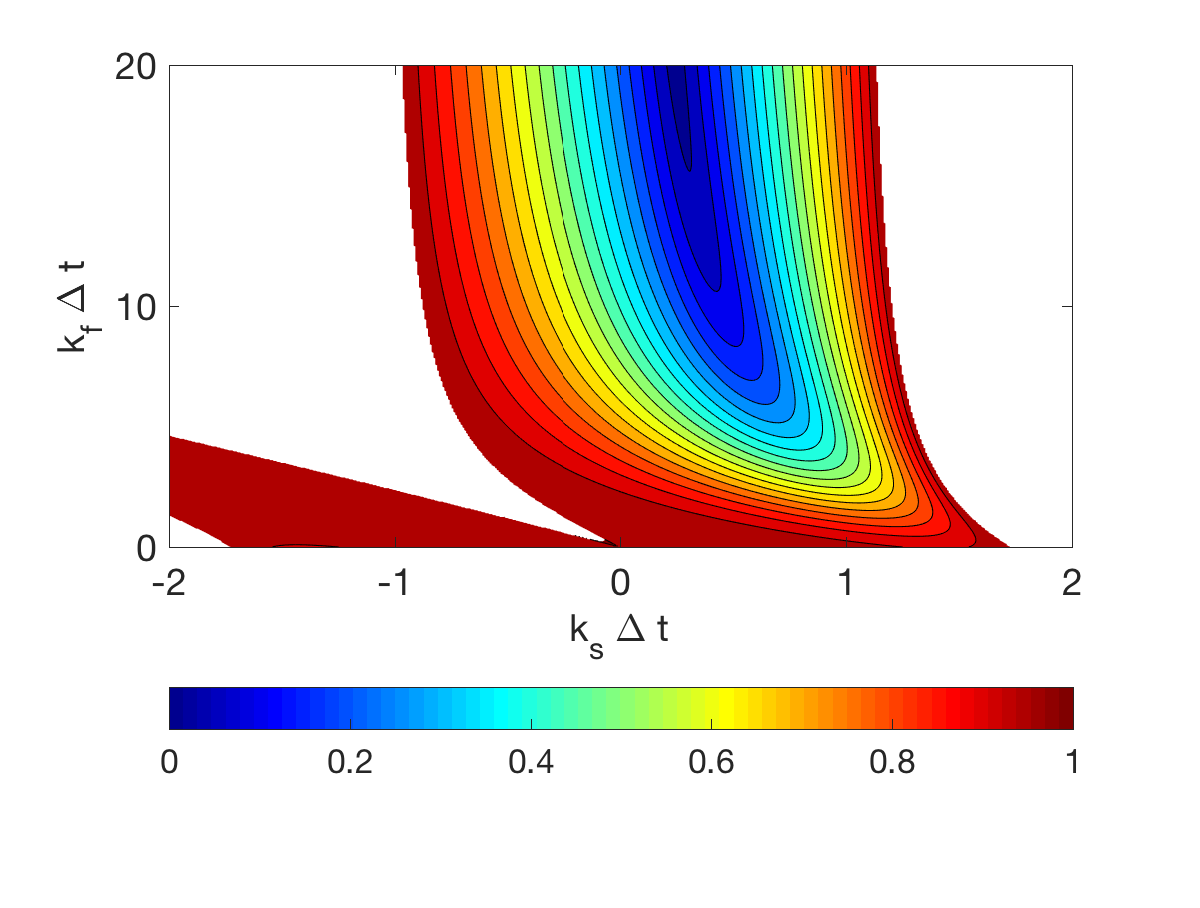
\includegraphics[width=1.5in]{figures/ARKA232_IMEX_Stability_ks=02_kf=20.eps}}
\subfigure[ARKB(2,3,2)]{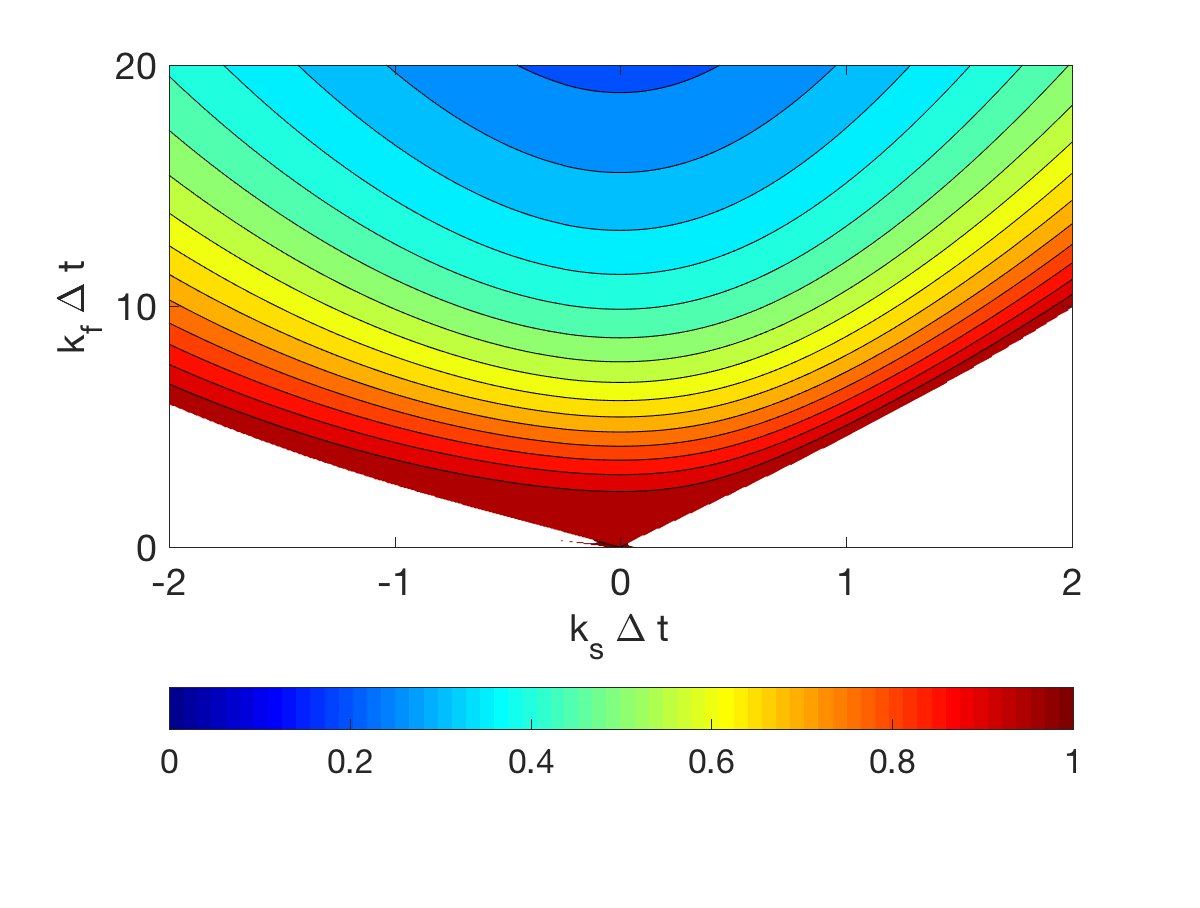
\includegraphics[width=1.5in]{figures/ARKB232_IMEX_Stability_ks=02_kf=20.eps}}
\subfigure[ARK(1,2,1)]{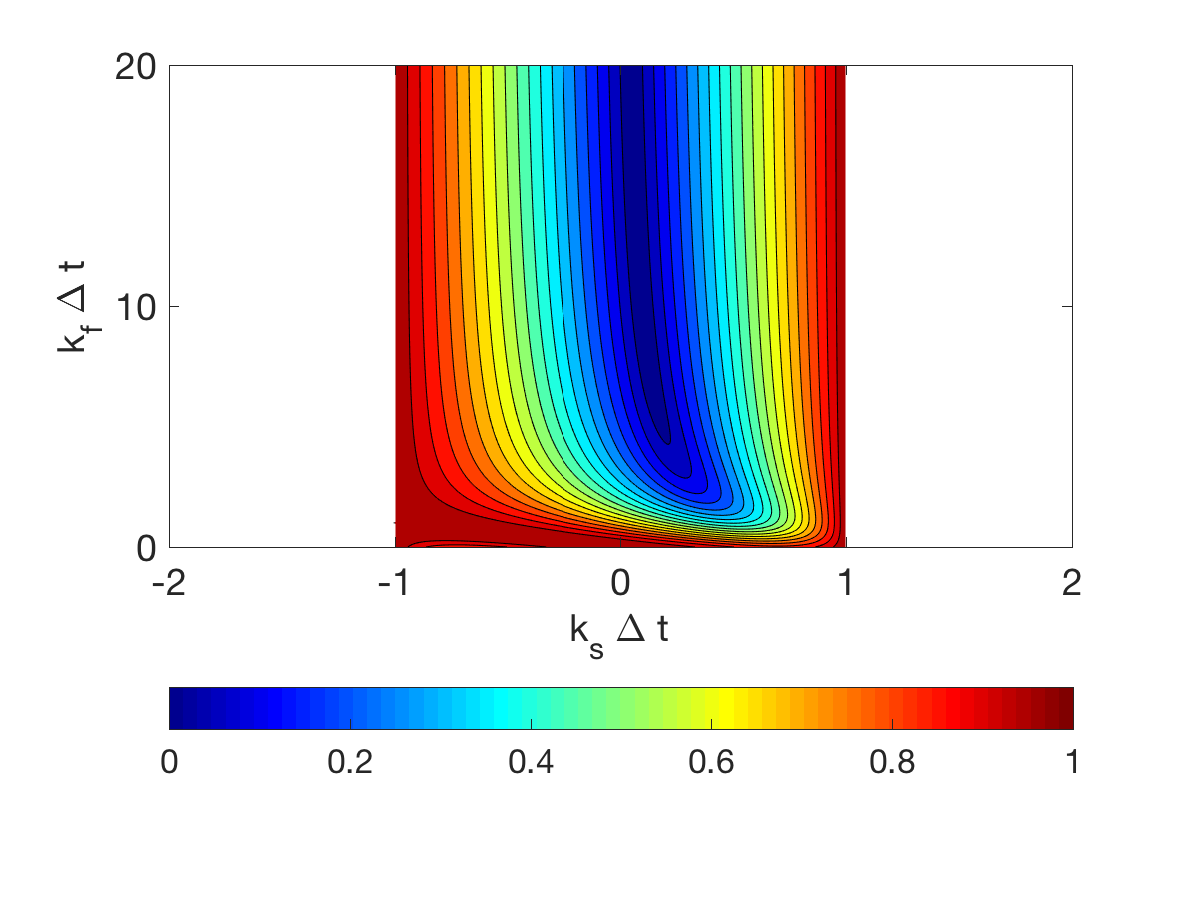
\includegraphics[width=1.5in]{figures/ARK121_Stability_ks=02_kf=20.eps}}
\end{center}
\caption{Stability regions for ARKA(2,3,2), ARKB(2,3,2), and ARK(1,2,1) for $k_s \in [-2,2]$ and $k_f \in [0,20]$.}
\label{fig:time_integration/imex_stability}
\end{figure}
Note that ARKB(2,3,2) has the typical wedge-shape stability region where the explicit part of the stability region (horizontal axis) allows larger wave speeds for the slow component than expected as we handle larger wave speeds for the fast component (vertical axis).  However, this occurs because the waves are damped (e.g., blue region). In contrast, the ARKA(2,3,2) and ARK(1,2,1) methods are attractive because at the stability limit of the method (red region) we are able to get a solution that is not damped but at the cost of adhering to smaller wave speeds for the explicit (slow) component ($\lvert k_s \lvert < 2$); the advantage of ARKA(2,3,2) over ARK(1,2,1) is that the method is second order for nonlinear terms and third order for linear terms.
\begin{table}[htbp]
\caption{Butcher tableau for a second-order IMEX Runge-Kutta ARK(2,3,2) method.}
\centering
\begin{tabular}{c|cccc}
\ST 0 & 0 & & \\
 \ST $2 - \sqrt{2}$ & $2-\sqrt{2}$ & 0 &  \\
 \ST $1$ & $1- a_{32}$  &  $a_{32}$ &  $0$  \\
 \hline
\ST  & $\frac{1}{2\sqrt{2}}$ &  $\frac{1}{2\sqrt{2}}$ & $1 - \frac{1}{\sqrt{2}}$ \\
\end{tabular}
\hspace{0.25in}
\begin{tabular}{c|cccc}
\ST 0 & 0 & & \\
 \ST $2 - \sqrt{2}$ & $1-\frac{1}{\sqrt{2}}$ & $1-\frac{1}{\sqrt{2}}$ &  \\
 \ST $1$ & $\frac{1}{2\sqrt{2}}$  &  $\frac{1}{2\sqrt{2}}$ &  $1 - \frac{1}{\sqrt{2}}$  \\
 \hline
\ST  & $\frac{1}{2\sqrt{2}}$ &  $\frac{1}{2\sqrt{2}}$ & $1 - \frac{1}{\sqrt{2}}$ \\
\end{tabular}
\label{table:time_integration/imex/ark232}
\end{table}
\begin{table}[ht]
\caption{Butcher tableau for a first-order IMEX Runge-Kutta ARK(1,2,1) method.}
\centering
\begin{tabular}{c|cccc}
\ST 0 && 0 && \\
 \ST $1$ && $1$ && 0  \\
 \hline
\ST  && 0 &&  $1$ \\
\end{tabular}
\hspace{0.5in}
\begin{tabular}{c|cccc}
\ST 0 &&  0 &&  \\
 \ST $1$ && 0 && $1$  \\
 \hline
\ST  && 0 &&  $1$ \\
\end{tabular}
\label{table:time_integration/imex/ark121}
\end{table}
\clearpage

\section{Fully Explicit Multirate Method: Substepping}
\label{sec:substepping}

\subsection{Split-Explicit as in Wicker-Skamarock}
To discretize the equations in time using a simple partitioned Runge-Kutta method (as in Wicker-Skamarock MWR 2002), let us describe the method using the following 3-partition system of ordinary differential equations:
\[
\diff{\vec{Y}}{t}= L_I(\vec{Y}) + \Tvector_{d'} + \Tvector_{-s}
\]
where $\Tvector_{d'}=\Tvector^N_{I}(\vec{Y}) + \Tvector_{d}$, and the right-hand side is ordered in ascending wave-speed order, i.e., 
the wave speed $\mathcal{S}$ of the different components are ordered as follows $\mathcal{S}(L_I) > \mathcal{S}(\Tvector_{d'})$, etc.

The algorithm describing the 3-partition multirate RK method is highlighted in Alg.\ \ref{alg:split-explicit-WS2002}.
\comment{
\begin{algorithm}
\label{alg:4-prk}
\begin{algorithmic}
\State
\Function{4-Partition Multirate RK}{}
\State update $\Tvector_{-s}(\magenta{ \vec{Y}^{n-s}})$
\State $\vec{Y}^{(i)}=\vec{Y}^n$ 
\For{$i=1:I$} 
\State $\vec{Y}^{(j)}=\vec{Y}^{(i)}$ \Comment update $\Tvector_{d'}(\red{ \vec{Y}^{(i)} })$
\For{$j=1:J$} 
\State $\vec{Y}^{(k)}=\vec{Y}^{(j)}$ \Comment update $\Tvector_{+f}(\blue{ \vec{Y}^{(j)} })$
\For{$k=1:K$} 
\State $\vec{Y}^{(k)}=\vec{Y}^{(j)} + \Delta \tau \left[ \Tvector_{-s}(\magenta{ \vec{Y}^{n-s} }) + \Tvector_{d'}(\red{ \vec{Y}^{(i)}}) + \Tvector_{+f}(\blue{ \vec{Y}^{(j)} }) + L_I(\vec{Y}^{(k)}) \right]$
\EndFor %k
\State $\vec{Y}^{(j)}=\vec{Y}^{(k)}$
\EndFor %j
\State $\vec{Y}^{(i)}=\vec{Y}^{(j)}$
\EndFor %i
\State $\vec{Y}^{n+1}=\vec{Y}^{(i)}$
\EndFunction
\end{algorithmic}
\end{algorithm}
}
\begin{algorithm}
\label{alg:split-explicit-WS2002}
\begin{algorithmic}
\State
\Function{3-Partition Split-Explicit General RK}{}
\State update $\Tvector_{-s}(\magenta{ \vec{Y}^{n-s}})$
\State $\vec{Y}^{(i)}=\vec{Y}^n$ 
\For{$i=2:I+1$} 
\State update $\Tvector_{d'}(\red{ \vec{Y}^{(i)} })$
\State $\vec{Y}^{(m)}=\vec{Y}^{n}$ 
\For{$m=1:c_i \cdot M$} 
\State $\vec{Y}^{(m)}=\vec{Y}^{(m)} + \frac{\Delta t}{M} \left[ \Tvector_{-s}(\magenta{ \vec{Y}^{n-s} }) + \Tvector_{d'}(\red{ \vec{Y}^{(i)}}) + L_I(\vec{Y}^{(m)}) \right]$
\EndFor %k
\State $\vec{Y}^{(i)}=\vec{Y}^{(m)}$
\EndFor %i
\State $\vec{Y}^{n+1}=\vec{Y}^{(i)}$
\EndFunction
\end{algorithmic}
\end{algorithm}
In Alg.\ \ref{alg:split-explicit-WS2002} the red and magenta fonts indicate terms that are frozen within the $m$-loop and is what allows a performance gain since these terms are not computed within this loop. Also, 
the RK coefficients are written in low-storage form as follows $a_{i+1}=\frac{1}{I-i+1}$ with $c_i=a_i$. Unfortunately, this approach only yields a convergence rate of 1 since the inner loop uses forward Euler.

\comment{
If all partitions are of the same order then the effective time-step of each partition is 
\[
\mathcal{O} \left( \frac{\Delta t}{N_{RK}^{p-1}} \right)
\]where $N_{RK}$ is the order of the RK method and $p$ refers to the partition (e.g., for $p=1$ the time-step is $\Delta t$, for $p=2$ the time-step is $\Delta t/N_{RK}$, and for $p=3$ the time-step is $\Delta t/N_{RK}^2$). 

If the embedded partition described in Alg.\ \ref{alg:4-prk} yields an insufficiently small time-step to maintain stability of the fastest waves then substepping can be added as shown in Alg.\ \ref{alg:4-prk_v2} where an additional loop ($m$-loop) is inserted before the $k$-loop.
\begin{algorithm}
\label{alg:4-prk_v2}
\begin{algorithmic}
\State
\Function{4-Partition Multirate RK with Euler Substepping}{}
\State update $\Tvector_{-s}(\magenta{ \vec{Y}^{n-s}})$
\State $\vec{Y}^{(i)}=\vec{Y}^n$ 
\For{$i=1:I$} 
\State $\vec{Y}^{(j)}=\vec{Y}^{(i)}$ \Comment update $\Tvector_{d'}(\red{ \vec{Y}^{(i)} })$
\For{$j=1:J$} 
\State $\vec{Y}^{(m)}=\vec{Y}^{(j)}$ \Comment update $\Tvector_{+f}(\blue{ \vec{Y}^{(j)} })$
\For{$m=1:M$} 
\State $\vec{Y}^{(k)}=\vec{Y}^{(m)}$
\For{$k=1:K$} 
\State $\vec{Y}^{(k)}=\vec{Y}^{(m)} + \Delta \tau \left[ \Tvector_{-s}(\magenta{ \vec{Y}^{n-s} }) + \Tvector_{d'}(\red{ \vec{Y}^{(i)}}) + \Tvector_{+f}(\blue{ \vec{Y}^{(j)} }) + L_I(\vec{Y}^{(k)}) \right]$
\EndFor %k
\State $\vec{Y}^{(m)}=\vec{Y}^{(k)}$
\EndFor %m
\State $\vec{Y}^{(j)}=\vec{Y}^{(m)}$
\EndFor %j
\State $\vec{Y}^{(i)}=\vec{Y}^{(j)}$
\EndFor %i
\State $\vec{Y}^{n+1}=\vec{Y}^{(i)}$
\EndFunction
\end{algorithmic}
\end{algorithm}
In Alg.\ \ref{alg:4-prk_v2}
$\Delta \tau=\frac{\Delta t}{M} a_i^I a_j^J a_k^K$.
}

\subsection{Multirate as in Wensch-Knoth}
The approach presented previously has been used in various nonhydrostatic codes and has been shown to work effectively to increase the time-to-solution of the problem.  However, the Butcher tableaux required in that approach is rather limited (only one type of RK method was originally proposed and forward Euler was used in the inner/fast loop which is not ideal for high-order spatial discretization methods).  A general approach was introduced by Wensch and Knoth in order to give split-explicit methods a more formal mathematical formulation.  Wensch and Knoth generalized this approach further to yield multirate methods that have better than 1st order convergence rates which we now describe in Alg.\ \ref{alg:general_explicit_multirate} for the following three-partitioned equation
\[
\diff{\vec{Y}}{t}= L_I(\vec{Y}) +  \Tvector_{d'} + \Tvector_{-s}.
\]
\begin{algorithm}
\label{alg:general_explicit_multirate}
\begin{algorithmic}
\State
\Function{3-Partition General Explicit Multirate RK}{}
\State $\vec{Q}^{(1)}=\vec{Y}^n$ 
\For{$i=2:I+1$} 
\State $\red{r_i}=\Tvector_{-s}(\magenta{ \vec{Y}^{n-s}}) + \sum_{j=1}^{i-1} \widetilde{a}_{i,j} \Tvector_{d'}(\red{\vec{Q}^{(1)}})$
\State $\vec{V}_{i,1}=\vec{Q}^{(i-1)}$
\For{$j=2:J+1$} 
\State $\vec{V}_{i,j}=\vec{V}_{i,j-1} + \Delta t \sum_{k=1}^{j-1} \widetilde{a}_{j,k} \left[ \red{r_i} + \widetilde{c}_{i} L_I(\vec{V}_{i,k}) \right]$ 
\EndFor %j
\State $\vec{Q}^{(i)}=\vec{V}_{i,J+1}$
\EndFor %i
\State $\vec{Y}^{n+1}=\vec{Q}^{(I+1)}$
\EndFunction
\end{algorithmic}
\end{algorithm}
where 
\[
\widetilde{a}_{i,j}=\left\{
\begin{array}{cc}
  {a}_{i,j}-{a}_{i-1,j}   &  i < s+1 \\
  {b}_{j}-{a}_{s,j}   &  i = s+1  
\end{array}
\right.
\]
and
\[
\widetilde{c}_{i}=\left\{
\begin{array}{cc}
  {c}_{i}-{c}_{i-1}   &  i < s+1 \\
  1-{c}_{s}   &  i = s+1  
\end{array}
\right.
\]
with $a$, $b$, and $c$ being the Butcher tableau coefficients found in Eq.\ \eqref{eq:butcher_tableau} and $s$ denotes the number of stages.  The only constraint on this algorithm is that the coefficients $c$ increase monotonically. If they do not, we can still use this approach but Alg.\ \ref{alg:general_explicit_multirate} would have to be modified.  Using this approach, the order of the scheme is min(order(I),order(J)) where  order(I) and order(J) are the orders of the RK methods with respect to the $I$ and $J$ loops.

\subsection{Multirate as in Wensch-Knoth for Low-Storage Methods}
Algorithm \ref{alg:general_explicit_multirate} represents a general multirate time-integration form that can be used with any comnbination of methods provided that they are written in Butcher tableau form.  However, the Butcher form requires the storage of stage values which may not be ideal on GPUs. Instead, we now rewrite this algorithm for low-storage RK methods which we describe below.
\begin{algorithm}
\label{alg:general_explicit_multirate/lsrk}
\begin{algorithmic}
\State
\Function{3-Partition General Explicit Multirate LSRK}{}
\State $\vec{y}=\vec{Y}^n$ 
\For{$i=1:I$} 
\State $\red{r_{slow}}=\Tvector_{-s}(\magenta{ \vec{Y}^{n-s}}) + A_i r_{slow} + \Tvector_{d'}(\red{\vec{y}})$
\State $\widetilde{c}_i=c_i - c_{i-1}$
\For{$j=1:J$} 
\State $r_{fast}=A_j r_{fast} + L_I(\vec{y}) + \frac{B_i}{c_i - c_{i-1}} \red{r_{slow}}$ 
\State $\vec{y} = \vec{y} + \Delta t \widetilde{c}_i  B_j r_{fast}$
\EndFor %j
\EndFor %i
\EndFunction
\end{algorithmic}
\end{algorithm}
The multirate LSRK presented in Alg.\  \ref{alg:general_explicit_multirate/lsrk} is the method currently implemented in CLIMA where the 5-stage (Kennedy-Carpenter) and 14-stage (Niegemann et al.) LSRK methods are included, where the coefficients $A$ and $B$ are the typical coefficients in Williamson low-storage form.

\section{Stability of Explicit Methods in CLIMA}
Figure \ref{fig:time_integration/explicit_stability} shows the explicit stability region of some of the time-integrators available in CLIMA; for comparison, the classical RK4 is included.  Figure \ref{fig:time_integration/explicit_stability}(a) shows the stability region per-stage whereas \ref{fig:time_integration/explicit_stability}(b) shows the total stability region.  In these figures, the vertical axis represents the stability for thd non-dissipative components (e.g., 1st order hyperbolic operators) whereas the horizontal axis the dissipative components (e.g., second order elliptic operators and the dissipation introduced by the Rusanov numerical flux).  Although we cannot use these figures to predict the exact Courant numbers for each of the methods, we can use these figures to get a sense of the difference in the stability regions for each of the time-integrators. For example, we can see that the explicit tableau for the IMEX ARK(2,3,2) method is much smaller than that for the LSRK(14,4) method. In fact, Fig.\ \ref{fig:time_integration/explicit_stability}(b) shows that the LSRK(14,4) method has a particularly large stability region (compared to the other methods) for the dissipative components.
\begin{figure}[htbp]
\begin{center}
\subfigure[Per-stage Stability]{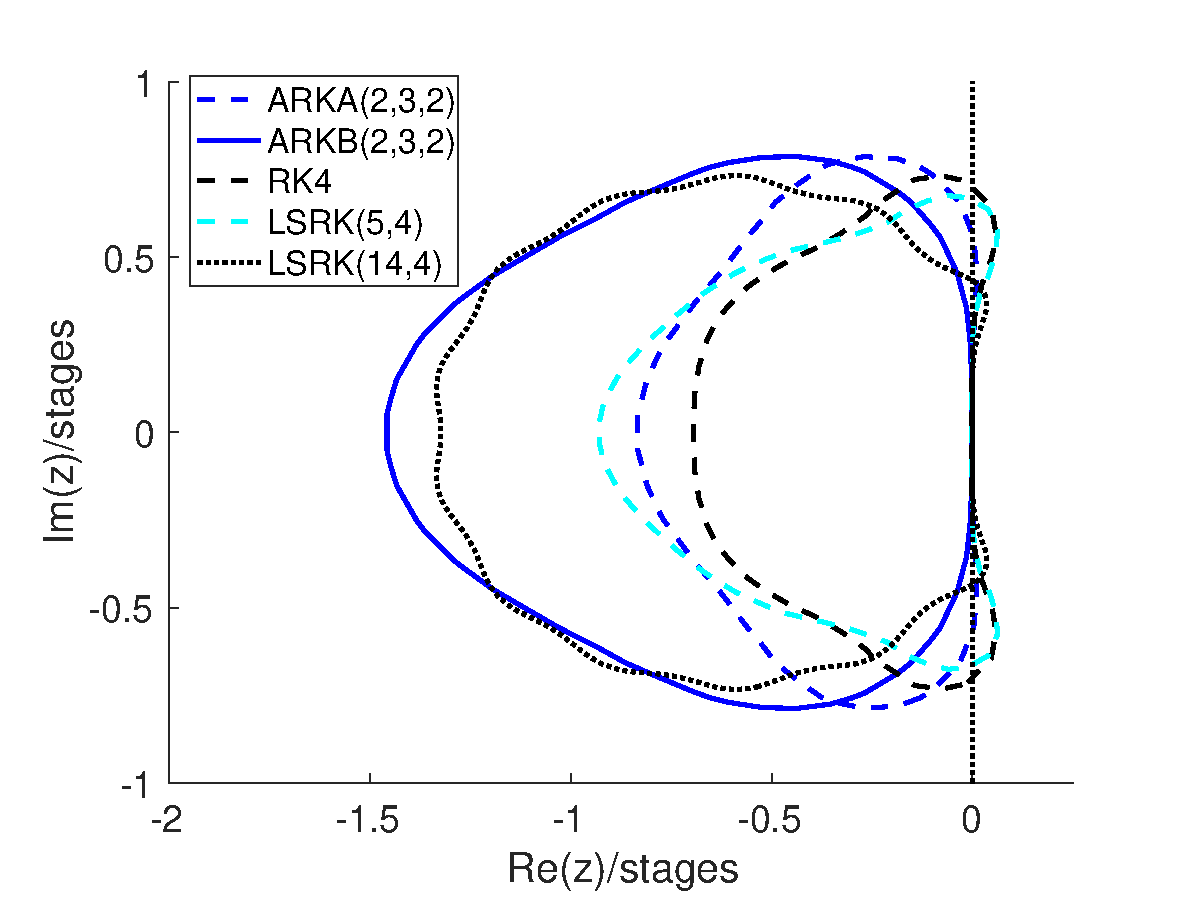
\includegraphics[width=2.25in]{figures/Stability_CLIMA_RK_Methods_Per_stage_Stability.eps}}
\subfigure[Total Stability]{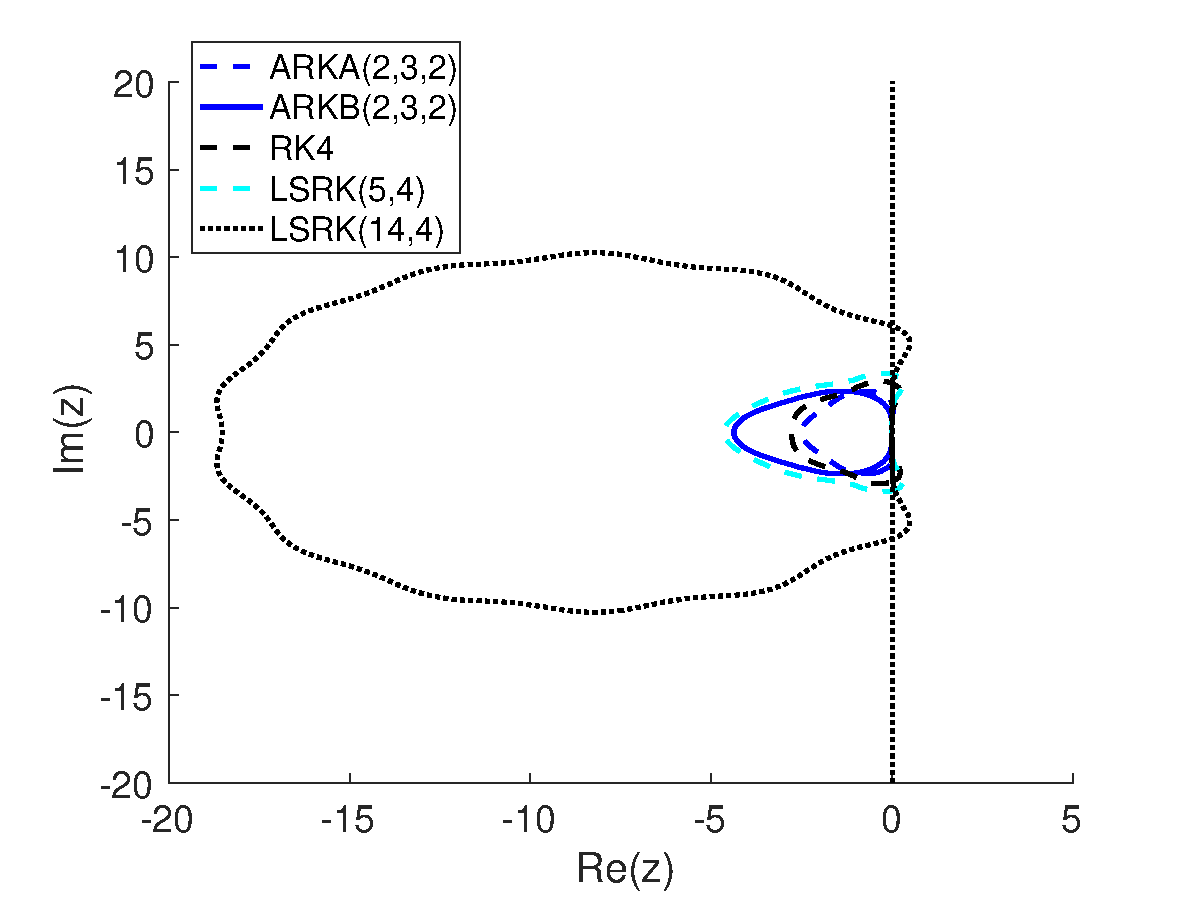
\includegraphics[width=2.25in]{figures/Stability_CLIMA_RK_Methods_Total_Stability.eps}}
\end{center}
\caption{Explicit stability regions for the some time-integrators in CLIMA. Panel (a) shows the stability region per stage while panel (b) shows the total stability region.
\hlc[green]{Toby: I think one section we need here and that would be useful generally is would contain rules of thumb for the best stable Courant number based on horizontal spacing for each time stepping method used in the ClIMA code. Example: Currently, as default, we use a 1D-IMEX with the ARK2GKC time stepper and a courant number of 0.4. One can see this in the CLIMA master branch src/Driver/Driver.jl l.210 and src/Driver/Configurations.jl l.31. I think having this in the design doc and matching the codebase would be fantastic}
}
\fxg{Thomas is working on this}
\label{fig:time_integration/explicit_stability}
\end{figure}

\section{Guidelines for Selecting the Time-Step}
The time-step restriction for an explicit method must satisfy the stable Courant number for the specific time-integrator and must be selected from the following constraints
\[
\Delta t_{\mathrm{explicit}} = min \left( \frac{C \Delta s_i}{u_i + a}, \frac{C \Delta s_i^2}{\nu} \right)
\]
where $C$ is the stable Courant number, $u_i$ denotes the velocity components, $a$ the speed of sound, $\Delta s_i$ the grid spacing along the direction ($x_1,x_2,x_3$), and $\nu$ the kinematic viscosity. The first term on the right is the time-step condition due to the non-dissipative components while the second term to the dissipation. For explicit time-integrators, we have to find the minimum time-step that satisfies this condition along all three spatial directions.

In the case of 3D-IMEX, the largest stable time-step is obtained from the conditions
\[
\Delta t_{\mathrm{3D-IMEX}} = min \left( \frac{C \Delta s_i}{u_i}, \frac{C \Delta s_i^2}{\nu} \right)
\]
where we now are unconditionally stable with respect to the speed of sound (since these terms are solved implicitly) and where we assume here that the diffusion is handled fully explicitly.

In the case of 1D-IMEX along the vertical direction, the largest stable time-step is obtained from the conditions
\[
\Delta t_{\mathrm{1D-IMEX}} = min \left( \frac{C \Delta s_H}{u_H+a}, \frac{C \Delta s_V}{u_V}, \frac{C \Delta s^2}{\nu} \right)
\]
where the subscripts $H$ and $V$ denote the \emph{horizontal} and \emph{vertical} components. Again,here we assume that the viscosity is handled fully explicitly.

\hl{Akshay: We currently have MultirateRungeKutta.jl which allows a model to be split into its fast / slow components (we have the isentropic vortex example demonstrating use of this, and I have an example with the Rayleigh-Benard case with two explicit rates, and an LES example with IMEX + 1 horizontal rate: (a)does the current setup allow us to use more than 2 rates in the horizontal (if so, where in the source code should I be looking? (We'd like to move towards vertical implicit solve + 2 horizontal explicit rates) (b)The explicit solver type supported by MultirateRungeKutta is restricted to the LSRK2N type; is this the recommended solver in the default case given the stability margins? (c)The CFL calculator would help in setting up a general method for multirate timestepping. (see solver setup() in Driver.jl))?}
\fxg{Akshay, let me check on this for you.}
%-------Bibliography
\bibliographystyle{agufull08}
\bibliography{Giraldo_refs,CLIMA-refs}

\end{document}
